\documentclass[12pt]{article}
\usepackage{fontspec}
\usepackage{fullpage}
\usepackage{hyperref}
\hypersetup{bookmarks=true,colorlinks=true,linkcolor=red,citecolor=blue,filecolor=magenta,urlcolor=cyan}
\usepackage{amsmath}
\usepackage{amssymb}
\usepackage{mathtools}
\usepackage{unicode-math}
\usepackage{tabu}
\usepackage{longtable}
\usepackage{booktabs}
\usepackage{caption}
\usepackage{graphics}
\usepackage{enumitem}
\usepackage{filecontents}
\usepackage[backend=bibtex]{biblatex}
\usepackage{url}
\setmathfont{Latin Modern Math}
\newcommand{\gt}{\ensuremath >}
\newcommand{\lt}{\ensuremath <}
\global\tabulinesep=1mm
\newlist{symbDescription}{description}{1}
\setlist[symbDescription]{noitemsep, topsep=0pt, parsep=0pt, partopsep=0pt}
\bibliography{bibfile}
\title{Software Requirements Specification for Game Physics}
\author{Alex Halliwushka, Luthfi Mawarid, and Olu Owojaiye}
\begin{document}
\maketitle
\tableofcontents
\newpage
\section{Reference Material}
\label{Sec:RefMat}
This section records information for easy reference.

\subsection{Table of Units}
\label{Sec:ToU}
The unit system used throughout is SI (Système International d'Unités). In addition to the basic units, several derived units are also used. For each unit, the \hyperref[Table:ToU]{table of units} lists the symbol, a description and the SI name.

\begin{longtable}{l l l}
\toprule
\textbf{Symbol} & \textbf{Description} & \textbf{SI Name}
\\
\midrule
\endhead
${\text{J}}$ & energy & joule
\\
${\text{kg}}$ & mass & kilogram
\\
${\text{m}}$ & length & metre
\\
${\text{N}}$ & force & newton
\\
${\text{rad}}$ & angle & radian
\\
${\text{s}}$ & time & second
\\
\bottomrule
\caption{Table of Units}
\label{Table:ToU}
\end{longtable}
\subsection{Table of Symbols}
\label{Sec:ToS}
The symbols used in this document are summarized in the \hyperref[Table:ToS]{table of symbols} along with their units. Throughout the document, symbols in bold will represent vectors, and scalars otherwise. The symbols are listed in alphabetical order. For vector quantities, the units shown are for each component of the vector.

\begin{longtabu}{l X[l] l}
\toprule
\textbf{Symbol} & \textbf{Description} & \textbf{Units}
\\
\midrule
\endhead
$\mathbf{a}$ & Acceleration & $\frac{\text{m}}{\text{s}^{2}}$
\\
$\mathbf{a}\text{(}t\text{)}$ & Linear acceleration & $\frac{\text{m}}{\text{s}^{2}}$
\\
${\mathbf{a}_{j}}$ & J-Th Body's Acceleration & $\frac{\text{m}}{\text{s}^{2}}$
\\
${C_{\text{R}}}$ & Coefficient of restitution & --
\\
${d_{j}}$ & Distance Between the J-Th Particle and the Axis of Rotation & ${\text{m}}$
\\
$\mathbf{d}$ & Distance between the center of mass of the rigid bodies & ${\text{m}}$
\\
$\mathbf{\hat{d}}$ & Unit vector directed from the center of the large mass to the center of the smaller mass & ${\text{m}}$
\\
$\mathbf{F}$ & Force & ${\text{N}}$
\\
${\mathbf{F}_{1}}$ & Force exerted by the first body (on another body) & ${\text{N}}$
\\
${\mathbf{F}_{2}}$ & Force exerted by the second body (on another body) & ${\text{N}}$
\\
${\mathbf{F}_{\mathbf{g}}}$ & Force of gravity & ${\text{N}}$
\\
${\mathbf{F}_{j}}$ & Force Applied to the J-Th Body at Time T & ${\text{N}}$
\\
$G$ & Gravitational constant & $\frac{\text{m}^{3}}{\text{kg}\text{s}^{2}}$
\\
$\mathbf{g}$ & Gravitational acceleration & $\frac{\text{m}}{\text{s}^{2}}$
\\
$h$ & Height & ${\text{m}}$
\\
$\mathbf{I}$ & Moment of inertia & $\text{kg}\text{m}^{2}$
\\
${\mathbf{I}_{\text{A}}}$ & Moment of Inertia of Rigid Body A & $\text{kg}\text{m}^{2}$
\\
${\mathbf{I}_{\text{B}}}$ & Moment of Inertia of Rigid Body B & $\text{kg}\text{m}^{2}$
\\
$\mathbf{J}$ & Impulse (vector) & $\text{N}\text{s}$
\\
$j$ & Impulse (scalar) & $\text{N}\text{s}$
\\
$KE$ & Kinetic energy & ${\text{J}}$
\\
$L$ & Length & ${\text{m}}$
\\
$M$ & Mass of the Larger Rigid Body & ${\text{kg}}$
\\
$m$ & Mass & ${\text{kg}}$
\\
${m_{1}}$ & Mass of the first body & ${\text{kg}}$
\\
${m_{2}}$ & Mass of the second body & ${\text{kg}}$
\\
${m_{\text{A}}}$ & Mass of Rigid Body A & ${\text{kg}}$
\\
${m_{\text{B}}}$ & Mass of Rigid Body B & ${\text{kg}}$
\\
${m_{j}}$ & Mass of the J-Th Particle & ${\text{kg}}$
\\
${m_{T}}$ & Total Mass of the Rigid Body & ${\text{kg}}$
\\
$\mathbf{n}$ & Collision normal vector & ${\text{m}}$
\\
$PE$ & Potential energy & ${\text{J}}$
\\
$\mathbf{p}$ & Position & ${\text{m}}$
\\
${\mathbf{p}_{\text{CM}}}$ & Center of Mass & ${\text{m}}$
\\
${\mathbf{p}_{j}}$ & Position Vector of the J-Th Particle & ${\text{m}}$
\\
$\mathbf{r}$ & Position vector & ${\text{m}}$
\\
$t$ & Time & ${\text{s}}$
\\
${t_{\text{c}}}$ & Denotes the time at collision & ${\text{s}}$
\\
$\mathbf{u}$ & Displacement & ${\text{m}}$
\\
$\mathbf{u}\text{(}t\text{)}$ & Linear displacement & ${\text{m}}$
\\
${\mathbf{u}_{\text{O}\text{B}}}$ & Displacement vector between the origin and point B & ${\text{m}}$
\\
$\mathbf{v}$ & Velocity & $\frac{\text{m}}{\text{s}}$
\\
$Δ\mathbf{v}$ & Change in velocity & $\frac{\text{m}}{\text{s}}$
\\
$\mathbf{v}\text{(}t\text{)}$ & Linear velocity & $\frac{\text{m}}{\text{s}}$
\\
${\mathbf{v}^{\text{A}\text{P}}}$ & Velocity of the Point of Collision P in Body A & $\frac{\text{m}}{\text{s}}$
\\
${\mathbf{v}^{\text{B}\text{P}}}$ & Velocity of the Point of Collision P in Body B & $\frac{\text{m}}{\text{s}}$
\\
${\mathbf{v}_{1}}$ & Velocity of the First Body & $\frac{\text{m}}{\text{s}}$
\\
${\mathbf{v}_{2}}$ & Velocity of the Second Body & $\frac{\text{m}}{\text{s}}$
\\
${\mathbf{v}_{\text{A}}}$ & Velocity at Point A & $\frac{\text{m}}{\text{s}}$
\\
${\mathbf{v}_{\text{B}}}$ & Velocity at Point B & $\frac{\text{m}}{\text{s}}$
\\
${{\mathbf{v}_{\text{f}}}^{\text{A}\text{B}}}$ & Final Relative Velocity Between Rigid Bodies of A and B & $\frac{\text{m}}{\text{s}}$
\\
${{\mathbf{v}_{\text{i}}}^{\text{A}\text{B}}}$ & Initial Relative Velocity Between Rigid Bodies of A and B & $\frac{\text{m}}{\text{s}}$
\\
${\mathbf{v}_{j}}$ & Velocity of the J-Th Body's Velocity & $\frac{\text{m}}{\text{s}}$
\\
${\mathbf{v}_{\text{O}}}$ & Velocity at Point Origin & $\frac{\text{m}}{\text{s}}$
\\
$\text{||}\mathbf{d}\text{||}$ & Euclidean norm of the distance between the center of mass of two bodies & ${\text{m}}$
\\
$\text{||}\mathbf{n}\text{||}$ & Length of the normal vector & ${\text{m}}$
\\
$\text{||}{\mathbf{u}_{\text{A}\text{P}}}\text{*}\mathbf{n}\text{||}$ & Length of the Perpendicular Vector to the Contact Displacement Vector of Rigid Body A & ${\text{m}}$
\\
$\text{||}{\mathbf{u}_{\text{B}\text{P}}}\text{*}\mathbf{n}\text{||}$ & Length of the Perpendicular Vector to the Contact Displacement Vector of Rigid Body B & ${\text{m}}$
\\
${\text{||}\mathbf{d}\text{||}^{2}}$ & Squared distance & ${\text{m}^{2}}$
\\
$α$ & Angular acceleration & $\frac{\text{rad}}{\text{s}^{2}}$
\\
$θ$ & Angular displacement & ${\text{rad}}$
\\
$\mathbf{τ}$ & Torque & $\text{N}\text{m}$
\\
${\mathbf{τ}_{j}}$ & Torque applied to the j-th body & $\text{N}\text{m}$
\\
$ω$ & Angular velocity & $\frac{\text{rad}}{\text{s}}$
\\
$ϕ$ & Orientation & ${\text{rad}}$
\\
\bottomrule
\caption{Table of Symbols}
\label{Table:ToS}
\end{longtabu}
\subsection{Abbreviations and Acronyms}
\label{Sec:TAbbAcc}
\begin{longtable}{l l}
\toprule
\textbf{Abbreviation} & \textbf{Full Form}
\\
\midrule
\endhead
2D & Two-Dimensional
\\
3D & Three-Dimensional
\\
A & Assumption
\\
CM & Centre of Mass
\\
DD & Data Definition
\\
GD & General Definition
\\
GS & Goal Statement
\\
Game Physics & game physics library
\\
IM & Instance Model
\\
LC & Likely Change
\\
ODE & Ordinary Differential Equation
\\
R & Requirement
\\
SRS & Software Requirements Specification
\\
TM & Theoretical Model
\\
UC & Unlikely Change
\\
Uncert. & Typical Uncertainty
\\
\bottomrule
\caption{Abbreviations and Acronyms}
\label{Table:TAbbAcc}
\end{longtable}
\section{Introduction}
\label{Sec:Intro}
Due to the rising cost of developing video games, developers are looking for ways to save time and money for their projects. Using an open source physics library that is reliable and free will cut down development costs and lead to better quality products.

The following section provides an overview of the Software Requirements Specification (SRS) for Game Physics. This section explains the purpose of this document, the scope of the requirements, the characteristics of the intended reader, and the organization of the document.

\subsection{Purpose of Document}
\label{Sec:DocPurpose}
The primary purpose of this document is to record the requirements of the game physics library. Goals, assumptions, theoretical models, definitions, and other model derivation information are specified, allowing the reader to fully understand and verify the purpose and scientific basis of Game Physics. With the exception of \hyperref[Sec:SysConstraints]{system constraints}, this SRS will remain abstract, describing what problem is being solved, but not how to solve it.

This document will be used as a starting point for subsequent development phases, including writing the design specification and the software verification and validation plan. The design document will show how the requirements are to be realized, including decisions on the numerical algorithms and programming environment. The verification and validation plan will show the steps that will be used to increase confidence in the software documentation and the implementation. Although the SRS fits in a series of documents that follow the so-called waterfall model, the actual development process is not constrained in any way. Even when the waterfall model is not followed, as Parnas and Clements point out \cite{parnasClements1986}, the most logical way to present the documentation is still to ``fake'' a rational design process.

\subsection{Scope of Requirements}
\label{Sec:ReqsScope}
The scope of the requirements includes the physical simulation of 2D rigid bodies acted on by forces.

\subsection{Characteristics of Intended Reader}
\label{Sec:ReaderChars}
Reviewers of this documentation should have an understanding of rigid body dynamics and high school calculus. The users of Game Physics can have a lower level of expertise, as explained in \hyperref[Sec:UserChars]{Sec:User Characteristics}.

\subsection{Organization of Document}
\label{Sec:DocOrg}
The organization of this document follows the template for an SRS for scientific computing software proposed by \cite{koothoor2013} and \cite{smithLai2005}. The presentation follows the standard pattern of presenting goals, theories, definitions, and assumptions. For readers that would like a more bottom up approach, they can start reading the \hyperref[Sec:IMs]{instance models} and trace back to find any additional information they require.

The \hyperref[Sec:GoalStmt]{goal statements} are refined to the theoretical models and the \hyperref[Sec:TMs]{theoretical models} to the \hyperref[Sec:IMs]{instance models}.

\section{General System Description}
\label{Sec:GenSysDesc}
This section provides general information about the system. It identifies the interfaces between the system and its environment, describes the user characteristics, and lists the system constraints.

\subsection{System Context}
\label{Sec:SysContext}
\hyperref[Figure:sysCtxDiag]{Fig:sysCtxDiag} shows the system context. A circle represents an entity external to the software, the user in this case. A rectangle represents the software system itself (Game Physics). Arrows are used to show the data flow between the system and its environment.

\begin{figure}
\begin{center}
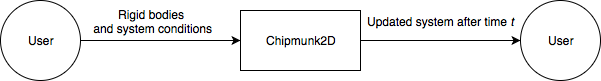
\includegraphics[width=\textwidth]{../../../datafiles/GamePhysics/sysctx.png}
\caption{System Context}
\label{Figure:sysCtxDiag}
\end{center}
\end{figure}
The interaction between the product and the user is through an application programming interface. The responsibilities of the user and the system are as follows:

\begin{itemize}
\item{User Responsibilities}
\begin{itemize}
\item{Provide initial conditions of the physical state of the simulation, rigid bodies present, and forces applied to them.}
\item{Ensure application programming interface use complies with the user guide.}
\item{Ensure required software assumptions (\hyperref[Sec:Assumps]{Sec:Assumptions}) are appropriate for any particular problem the software addresses.}
\end{itemize}
\item{Game Physics Responsibilities}
\begin{itemize}
\item{Determine if the inputs and simulation state satisfy the required physical and system constraints (\hyperref[Sec:DataConstraints]{Sec:Data Constraints}).}
\item{Calculate the new state of all rigid bodies within the simulation at each simulation step.}
\item{Provide updated physical state of all rigid bodies at the end of a simulation step.}
\end{itemize}
\end{itemize}
\subsection{User Characteristics}
\label{Sec:UserChars}
The end user of Game Physics should have an understanding of first year programming concepts and an understanding of high school physics.

\subsection{System Constraints}
\label{Sec:SysConstraints}
There are no system constraints.

\section{Specific System Description}
\label{Sec:SpecSystDesc}
This section first presents the problem description, which gives a high-level view of the problem to be solved. This is followed by the solution characteristics specification, which presents the assumptions, theories, and definitions that are used.

\subsection{Problem Description}
\label{Sec:ProbDesc}
A system is needed to create a simple, lightweight, fast, and portable 2D rigid body physics library, which will allow for more accessible game development and the production of higher quality products. Creating a gaming physics library is a difficult task. Games need physics libraries that simulate objects acting under various physical conditions, while simultaneously being fast and efficient enough to work in soft real-time during the game. Developing a physics library from scratch takes a long period of time and is very costly, presenting barriers of entry which make it difficult for game developers to include physics in their products. There are a few free, open source and high quality physics libraries available to be used for consumer products (\hyperref[Sec:offShelfSolns]{Sec:Off-The-Shelf Solutions}).

\subsubsection{Terminology and Definitions}
\label{Sec:TermDefs}
This subsection provides a list of terms that are used in the subsequent sections and their meaning, with the purpose of reducing ambiguity and making it easier to correctly understand the requirements.

\begin{itemize}
\item{Rigid body: A solid body in which deformation is neglected.}
\item{Elasticity: The ratio of the relative velocities of two colliding objects after and before a collision.}
\item{Centre of mass: The mean location of the distribution of mass of the object.}
\item{Cartesian coordinate system: A coordinate system that specifies each point uniquely in a plane by a set of numerical coordinates, which are the signed distances to the point from two fixed perpendicular oriented lines, measured in the same unit of length (from \cite{cartesianWiki}).}
\item{Right-handed coordinate system: A coordinate system where the positive z-axis comes out of the screen..}
\item{line: An interval between two points (from \cite{lineSource}).}
\item{point: An exact location, it has no size, only position (from \cite{pointSource}).}
\item{damping: An influence within or upon an oscillatory system that has the effect of reducing, restricting or preventing its oscillations (from \cite{dampingSource}).}
\end{itemize}
\subsubsection{Goal Statements}
\label{Sec:GoalStmt}
Given the kinematic properties, and forces (including any collision forces) applied on a set of rigid bodies, the goal statements are:

\begin{itemize}
\item[Determine-Linear-Properties:\phantomsection\label{linearGS}]{Determine their new positions and velocities over a period of time.}
\item[Determine-Angular-Properties:\phantomsection\label{angularGS}]{Determine their new orientations and angular velocities over a period of time.}
\end{itemize}
\subsection{Solution Characteristics Specification}
\label{Sec:SolCharSpec}
The instance models that govern Game Physics are presented in the \hyperref[Sec:IMs]{instance model section}. The information to understand the meaning of the instance models and their derivation is also presented, so that the instance models can be verified.

\subsubsection{Assumptions}
\label{Sec:Assumps}
This section simplifies the original problem and helps in developing the theoretical models by filling in the missing information for the physical system. The assumptions refine the scope by providing more detail.

\begin{itemize}
\item[objectTy:\phantomsection\label{assumpOT}]{All objects are rigid bodies. (RefBy: \hyperref[DD:chaslesThm]{DD:chaslesThm}, \hyperref[DD:reVeInColl]{DD:reVeInColl}, \hyperref[IM:rotMot]{IM:rotMot}, \hyperref[DD:potEnergy]{DD:potEnergy}, \hyperref[DD:ctrOfMass]{DD:ctrOfMass}, \hyperref[DD:momentOfInertia]{DD:momentOfInertia}, \hyperref[DD:linVel]{DD:linVel}, \hyperref[DD:linDisp]{DD:linDisp}, \hyperref[DD:linAcc]{DD:linAcc}, \hyperref[DD:kEnergy]{DD:kEnergy}, \hyperref[DD:impulseV]{DD:impulseV}, \hyperref[GD:impulse]{GD:impulse}, \hyperref[IM:col2D]{IM:col2D}, \hyperref[DD:angVel]{DD:angVel}, \hyperref[DD:angDisp]{DD:angDisp}, \hyperref[DD:angAccel]{DD:angAccel}, and \hyperref[IM:transMot]{IM:transMot}.)}
\item[objectDimension:\phantomsection\label{assumpOD}]{All objects are 2D. (RefBy: \hyperref[IM:rotMot]{IM:rotMot}, \hyperref[DD:potEnergy]{DD:potEnergy}, \hyperref[TM:NewtonSecLawRotMot]{TM:NewtonSecLawRotMot}, \hyperref[DD:kEnergy]{DD:kEnergy}, \hyperref[GD:impulse]{GD:impulse}, \hyperref[IM:col2D]{IM:col2D}, \hyperref[DD:angVel]{DD:angVel}, \hyperref[DD:angDisp]{DD:angDisp}, \hyperref[DD:angAccel]{DD:angAccel}, and \hyperref[IM:transMot]{IM:transMot}.)}
\item[coordinateSystemTy:\phantomsection\label{assumpCST}]{The library uses a Cartesian coordinate system.}
\item[axesDefined:\phantomsection\label{assumpAD}]{The axes are defined using right-handed coordinate system. (RefBy: \hyperref[IM:rotMot]{IM:rotMot}, \hyperref[GD:impulse]{GD:impulse}, and \hyperref[IM:col2D]{IM:col2D}.)}
\item[collisionType:\phantomsection\label{assumpCT}]{All rigid bodies collisions are vertex-to-edge collisions. (RefBy: \hyperref[lcEC]{LC:Expanded-Collisions}, \hyperref[GD:impulse]{GD:impulse}, and \hyperref[IM:col2D]{IM:col2D}.)}
\item[dampingInvolvement:\phantomsection\label{assumpDI}]{There is no damping involved throughout the simulation and this implies that there are no friction forces. (RefBy: \hyperref[DD:potEnergy]{DD:potEnergy}, \hyperref[lcID]{LC:Include-Dampening}, \hyperref[DD:kEnergy]{DD:kEnergy}, \hyperref[IM:col2D]{IM:col2D}, and \hyperref[IM:transMot]{IM:transMot}.)}
\item[constraintsAndJointsInvolvement:\phantomsection\label{assumpCAJI}]{There are no constraints and joints involved throughout the simulation. (RefBy: \hyperref[lcIJC]{LC:Include-Joints-Constraints}, \hyperref[IM:col2D]{IM:col2D}, and \hyperref[IM:transMot]{IM:transMot}.)}
\end{itemize}
\subsubsection{Theoretical Models}
\label{Sec:TMs}
This section focuses on the general equations and laws that Game Physics is based on.

\vspace{\baselineskip}
\noindent
\begin{minipage}{\textwidth}
\begin{tabular}{>{\raggedright}p{0.13\textwidth}>{\raggedright\arraybackslash}p{0.82\textwidth}}
\toprule \textbf{Refname} & \textbf{TM:NewtonSecLawMot}
\phantomsection 
\label{TM:NewtonSecLawMot}
\\ \midrule \\
Label & Newton's second law of motion
        
\\ \midrule \\
Equation & \begin{displaymath}
           \mathbf{F}=m \mathbf{a}
           \end{displaymath}
\\ \midrule \\
Description & \begin{symbDescription}
              \item{$\mathbf{F}$ is the force (${\text{N}}$)}
              \item{$m$ is the mass (${\text{kg}}$)}
              \item{$\mathbf{a}$ is the acceleration ($\frac{\text{m}}{\text{s}^{2}}$)}
              \end{symbDescription}
\\ \midrule \\
Notes & The net force $\mathbf{F}$ on a body is proportional to the acceleration $\mathbf{a}$ of the body, where $m$ denotes the mass of the body as the constant of proportionality.
        
\\ \midrule \\
Source & --
         
\\ \midrule \\
RefBy & \hyperref[IM:transMot]{IM:transMot}
        
\\ \bottomrule
\end{tabular}
\end{minipage}
\vspace{\baselineskip}
\noindent
\begin{minipage}{\textwidth}
\begin{tabular}{>{\raggedright}p{0.13\textwidth}>{\raggedright\arraybackslash}p{0.82\textwidth}}
\toprule \textbf{Refname} & \textbf{TM:NewtonThirdLawMot}
\phantomsection 
\label{TM:NewtonThirdLawMot}
\\ \midrule \\
Label & Newton's third law of motion
        
\\ \midrule \\
Equation & \begin{displaymath}
           {\mathbf{F}_{1}}=-{\mathbf{F}_{2}}
           \end{displaymath}
\\ \midrule \\
Description & \begin{symbDescription}
              \item{${\mathbf{F}_{1}}$ is the force exerted by the first body (on another body) (${\text{N}}$)}
              \item{${\mathbf{F}_{2}}$ is the force exerted by the second body (on another body) (${\text{N}}$)}
              \end{symbDescription}
\\ \midrule \\
Notes & Every action has an equal and opposite reaction. In other words, the force ${\mathbf{F}_{1}}$ exerted on the second rigid body by the first is equal in magnitude and in the opposite direction to the force ${\mathbf{F}_{2}}$ exerted on the first rigid body by the second.
        
\\ \midrule \\
Source & --
         
\\ \midrule \\
RefBy & 
\\ \bottomrule
\end{tabular}
\end{minipage}
\vspace{\baselineskip}
\noindent
\begin{minipage}{\textwidth}
\begin{tabular}{>{\raggedright}p{0.13\textwidth}>{\raggedright\arraybackslash}p{0.82\textwidth}}
\toprule \textbf{Refname} & \textbf{TM:UniversalGravLaw}
\phantomsection 
\label{TM:UniversalGravLaw}
\\ \midrule \\
Label & Newton's law of universal gravitation
        
\\ \midrule \\
Equation & \begin{displaymath}
           \mathbf{F}=G \frac{{m_{1}} {m_{2}}}{\text{||}\mathbf{d}\text{||}^{2}} \mathbf{\hat{d}}=G \frac{{m_{1}} {m_{2}}}{\text{||}\mathbf{d}\text{||}^{2}} \frac{\mathbf{d}}{\text{||}\mathbf{d}\text{||}}
           \end{displaymath}
\\ \midrule \\
Description & \begin{symbDescription}
              \item{$\mathbf{F}$ is the force (${\text{N}}$)}
              \item{$G$ is the gravitational constant ($\frac{\text{m}^{3}}{\text{kg}\text{s}^{2}}$)}
              \item{${m_{1}}$ is the mass of the first body (${\text{kg}}$)}
              \item{${m_{2}}$ is the mass of the second body (${\text{kg}}$)}
              \item{$\text{||}\mathbf{d}\text{||}$ is the Euclidean norm of the distance between the center of mass of two bodies (${\text{m}}$)}
              \item{$\mathbf{\hat{d}}$ is the unit vector directed from the center of the large mass to the center of the smaller mass (${\text{m}}$)}
              \item{$\mathbf{d}$ is the distance between the center of mass of the rigid bodies (${\text{m}}$)}
              \end{symbDescription}
\\ \midrule \\
Notes & Two rigid bodies in the universe attract each other with a force $\mathbf{F}$ that is directly proportional to the product of their masses, ${m_{1}}$ and ${m_{2}}$, and inversely proportional to the squared distance ${\text{||}\mathbf{d}\text{||}^{2}}$ between them.
        
\\ \midrule \\
Source & --
         
\\ \midrule \\
RefBy & \hyperref[GD:accelGravity]{GD:accelGravity}
        
\\ \bottomrule
\end{tabular}
\end{minipage}
\vspace{\baselineskip}
\noindent
\begin{minipage}{\textwidth}
\begin{tabular}{>{\raggedright}p{0.13\textwidth}>{\raggedright\arraybackslash}p{0.82\textwidth}}
\toprule \textbf{Refname} & \textbf{TM:NewtonSecLawRotMot}
\phantomsection 
\label{TM:NewtonSecLawRotMot}
\\ \midrule \\
Label & Newton's second law for rotational motion
        
\\ \midrule \\
Equation & \begin{displaymath}
           \mathbf{τ}=\mathbf{I} α
           \end{displaymath}
\\ \midrule \\
Description & \begin{symbDescription}
              \item{$\mathbf{τ}$ is the torque ($\text{N}\text{m}$)}
              \item{$\mathbf{I}$ is the moment of inertia ($\text{kg}\text{m}^{2}$)}
              \item{$α$ is the angular acceleration ($\frac{\text{rad}}{\text{s}^{2}}$)}
              \end{symbDescription}
\\ \midrule \\
Notes & The net torque $\mathbf{τ}$ on a rigid body is proportional to its angular acceleration $α$, where $\mathbf{I}$ denotes the moment of inertia of the rigid body as the constant of proportionality.
        
        We also assume that all rigid bodies involved are two-dimensional (from \hyperref[assumpOD]{A:objectDimension}).
        
\\ \midrule \\
Source & --
         
\\ \midrule \\
RefBy & \hyperref[IM:rotMot]{IM:rotMot}
        
\\ \bottomrule
\end{tabular}
\end{minipage}
\subsubsection{General Definitions}
\label{Sec:GDs}
This section collects the laws and equations that will be used to build the instance models.

\vspace{\baselineskip}
\noindent
\begin{minipage}{\textwidth}
\begin{tabular}{>{\raggedright}p{0.13\textwidth}>{\raggedright\arraybackslash}p{0.82\textwidth}}
\toprule \textbf{Refname} & \textbf{GD:accelGravity}
\phantomsection 
\label{GD:accelGravity}
\\ \midrule \\
Label & Acceleration due to gravity
        
\\ \midrule \\
Units & $\frac{\text{m}}{\text{s}^{2}}$
        
\\ \midrule \\
Equation & \begin{displaymath}
           \mathbf{g}=-\frac{G M}{\text{||}\mathbf{d}\text{||}^{2}} \mathbf{\hat{d}}
           \end{displaymath}
\\ \midrule \\
Description & \begin{symbDescription}
              \item{$\mathbf{g}$ is the gravitational acceleration ($\frac{\text{m}}{\text{s}^{2}}$)}
              \item{$G$ is the gravitational constant ($\frac{\text{m}^{3}}{\text{kg}\text{s}^{2}}$)}
              \item{$M$ is the mass of the larger rigid body (${\text{kg}}$)}
              \item{$\text{||}\mathbf{d}\text{||}$ is the Euclidean norm of the distance between the center of mass of two bodies (${\text{m}}$)}
              \item{$\mathbf{\hat{d}}$ is the unit vector directed from the center of the large mass to the center of the smaller mass (${\text{m}}$)}
              \end{symbDescription}
\\ \midrule \\
Notes & If one of the masses is much larger than the other, it is convenient to define a gravitational field around the larger mass as shown above. The negative sign in the equation indicates that the force is an attractive force.
        
\\ \midrule \\
Source & \hyperref{https://en.wikipedia.org/wiki/Gravitational_acceleration}{}{}{Definition of Gravitational Acceleration}
         
\\ \midrule \\
RefBy & \hyperref[IM:transMot]{IM:transMot}
        
\\ \bottomrule
\end{tabular}
\end{minipage}
\paragraph{Detailed derivation of gravitational acceleration:}
\label{GD:accelGravityDeriv}
From Newton's law of universal gravitation (\hyperref[TM:UniversalGravLaw]{TM:UniversalGravLaw}) we have:

\begin{displaymath}
\mathbf{F}=\frac{G {m_{1}} {m_{2}}}{{\text{||}\mathbf{d}\text{||}^{2}}} \mathbf{\hat{d}}
\end{displaymath}
The above equation governs the gravitational attraction between two bodies. Suppose that one of the bodies is significantly more massive than the other, so that we concern ourselves with the force the massive body exerts on the lighter body. Further, suppose that the Cartesian coordinate system is chosen such that this force acts on a line which lies along one of the principal axes. Then our unit vector directed from the center of the large mass to the center of the smaller mass $\mathbf{\hat{d}}$ for the x or y axes is:

\begin{displaymath}
\mathbf{\hat{d}}=\frac{\mathbf{d}}{\text{||}\mathbf{d}\text{||}}
\end{displaymath}
Given the above assumptions, let $M$ and $m$ be the mass of the massive and light body respectively. Equating $\mathbf{F}$ above with Newton's second law for the force experienced by the light body, we get:

\begin{displaymath}
{\mathbf{F}_{\mathbf{g}}}=G \frac{M m}{{\text{||}\mathbf{d}\text{||}^{2}}} \mathbf{\hat{d}}=m \mathbf{g}
\end{displaymath}
where $\mathbf{g}$ is the gravitational acceleration. Dividing the above equation by $m$,  we have:

\begin{displaymath}
G \frac{M}{{\text{||}\mathbf{d}\text{||}^{2}}} \mathbf{\hat{d}}=\mathbf{g}
\end{displaymath}
and thus the negative sign indicates that the force is an attractive force:

\begin{displaymath}
\mathbf{g}=-G \frac{M}{{\text{||}\mathbf{d}\text{||}^{2}}} \mathbf{\hat{d}}
\end{displaymath}
\vspace{\baselineskip}
\noindent
\begin{minipage}{\textwidth}
\begin{tabular}{>{\raggedright}p{0.13\textwidth}>{\raggedright\arraybackslash}p{0.82\textwidth}}
\toprule \textbf{Refname} & \textbf{GD:impulse}
\phantomsection 
\label{GD:impulse}
\\ \midrule \\
Label & Impulse for Collision
        
\\ \midrule \\
Units & $\text{N}\text{s}$
        
\\ \midrule \\
Equation & \begin{displaymath}
           j=\frac{-\left(1+{C_{\text{R}}}\right) {{\mathbf{v}_{\text{i}}}^{\text{A}\text{B}}}\cdot{}\mathbf{n}}{\left(\frac{1}{{m_{\text{A}}}}+\frac{1}{{m_{\text{B}}}}\right) \text{||}\mathbf{n}\text{||}^{2}+\frac{\text{||}{\mathbf{u}_{\text{A}\text{P}}}\text{*}\mathbf{n}\text{||}^{2}}{{\mathbf{I}_{\text{A}}}}+\frac{\text{||}{\mathbf{u}_{\text{B}\text{P}}}\text{*}\mathbf{n}\text{||}^{2}}{{\mathbf{I}_{\text{B}}}}}
           \end{displaymath}
\\ \midrule \\
Description & \begin{symbDescription}
              \item{$j$ is the impulse (scalar) ($\text{N}\text{s}$)}
              \item{${C_{\text{R}}}$ is the coefficient of restitution (Unitless)}
              \item{${{\mathbf{v}_{\text{i}}}^{\text{A}\text{B}}}$ is the initial relative velocity between rigid bodies of A and B ($\frac{\text{m}}{\text{s}}$)}
              \item{$\mathbf{n}$ is the collision normal vector (${\text{m}}$)}
              \item{${m_{\text{A}}}$ is the mass of rigid body A (${\text{kg}}$)}
              \item{${m_{\text{B}}}$ is the mass of rigid body B (${\text{kg}}$)}
              \item{$\text{||}\mathbf{n}\text{||}$ is the length of the normal vector (${\text{m}}$)}
              \item{$\text{||}{\mathbf{u}_{\text{A}\text{P}}}\text{*}\mathbf{n}\text{||}$ is the length of the perpendicular vector to the contact displacement vector of rigid body A (${\text{m}}$)}
              \item{${\mathbf{I}_{\text{A}}}$ is the moment of inertia of rigid body A ($\text{kg}\text{m}^{2}$)}
              \item{$\text{||}{\mathbf{u}_{\text{B}\text{P}}}\text{*}\mathbf{n}\text{||}$ is the length of the perpendicular vector to the contact displacement vector of rigid body B (${\text{m}}$)}
              \item{${\mathbf{I}_{\text{B}}}$ is the moment of inertia of rigid body B ($\text{kg}\text{m}^{2}$)}
              \end{symbDescription}
\\ \midrule \\
Notes & All bodies are assumed to be rigid (from \hyperref[assumpOT]{A:objectTy}) and two-dimensional (from \hyperref[assumpOD]{A:objectDimension}).
        
        A right-handed coordinate system is used (from \hyperref[assumpAD]{A:axesDefined}).
        
        All collisions are vertex-to-edge (from \hyperref[assumpCT]{A:collisionType}).
        
\\ \midrule \\
Source & \hyperref{http://www.chrishecker.com/images/e/e7/Gdmphys3.pdf}{}{}{Impulse for Collision Ref}
         
\\ \midrule \\
RefBy & \hyperref[IM:col2D]{IM:col2D}
        
\\ \bottomrule
\end{tabular}
\end{minipage}

\subsubsection{Data Definitions}
\label{Sec:DDs}
This section collects and defines all the data needed to build the instance models.

\vspace{\baselineskip}
\noindent
\begin{minipage}{\textwidth}
\begin{tabular}{>{\raggedright}p{0.13\textwidth}>{\raggedright\arraybackslash}p{0.82\textwidth}}
\toprule \textbf{Refname} & \textbf{DD:ctrOfMass}
\phantomsection 
\label{DD:ctrOfMass}
\\ \midrule \\
Label & Center of Mass
        
\\ \midrule \\
Symbol & ${\mathbf{p}_{\text{CM}}}$
         
\\ \midrule \\
Units & ${\text{m}}$
        
\\ \midrule \\
Equation & \begin{displaymath}
           {\mathbf{p}_{\text{CM}}}=\frac{\displaystyle\sum{{m_{j}} {\mathbf{p}_{j}}}}{{m_{T}}}
           \end{displaymath}
\\ \midrule \\
Description & \begin{symbDescription}
              \item{${\mathbf{p}_{\text{CM}}}$ is the Center of Mass (${\text{m}}$)}
              \item{${m_{j}}$ is the mass of the j-th particle (${\text{kg}}$)}
              \item{${\mathbf{p}_{j}}$ is the position vector of the j-th particle (${\text{m}}$)}
              \item{${m_{T}}$ is the total mass of the rigid body (${\text{kg}}$)}
              \end{symbDescription}
\\ \midrule \\
Notes & All bodies are assumed to be rigid (from \hyperref[assumpOT]{A:objectTy}).
        
\\ \midrule \\
Source & --
         
\\ \midrule \\
RefBy & \hyperref[IM:col2D]{IM:col2D} and \hyperref[IM:transMot]{IM:transMot}
        
\\ \bottomrule
\end{tabular}
\end{minipage}

\vspace{\baselineskip}
\noindent
\begin{minipage}{\textwidth}
\begin{tabular}{>{\raggedright}p{0.13\textwidth}>{\raggedright\arraybackslash}p{0.82\textwidth}}
\toprule \textbf{Refname} & \textbf{DD:linDisp}
\phantomsection 
\label{DD:linDisp}
\\ \midrule \\
Label & Linear displacement
        
\\ \midrule \\
Symbol & $\mathbf{u}\text{(}t\text{)}$
         
\\ \midrule \\
Units & ${\text{m}}$
        
\\ \midrule \\
Equation & \begin{displaymath}
           \mathbf{u}\text{(}t\text{)}=\frac{\,d\mathbf{p}\left(t\right)}{\,dt}
           \end{displaymath}
\\ \midrule \\
Description & \begin{symbDescription}
              \item{$\mathbf{u}\text{(}t\text{)}$ is the linear displacement (${\text{m}}$)}
              \item{$t$ is the time (${\text{s}}$)}
              \item{$\mathbf{p}$ is the position (${\text{m}}$)}
              \end{symbDescription}
\\ \midrule \\
Notes & All bodies are assumed to be rigid (from \hyperref[assumpOT]{A:objectTy}).
        
\\ \midrule \\
Source & --
         
\\ \midrule \\
RefBy & \hyperref[IM:transMot]{IM:transMot}
        
\\ \bottomrule
\end{tabular}
\end{minipage}

\vspace{\baselineskip}
\noindent
\begin{minipage}{\textwidth}
\begin{tabular}{>{\raggedright}p{0.13\textwidth}>{\raggedright\arraybackslash}p{0.82\textwidth}}
\toprule \textbf{Refname} & \textbf{DD:linVel}
\phantomsection 
\label{DD:linVel}
\\ \midrule \\
Label & Linear velocity
        
\\ \midrule \\
Symbol & $\mathbf{v}\text{(}t\text{)}$
         
\\ \midrule \\
Units & $\frac{\text{m}}{\text{s}}$
        
\\ \midrule \\
Equation & \begin{displaymath}
           \mathbf{v}\text{(}t\text{)}=\frac{\,d\mathbf{u}\left(t\right)}{\,dt}
           \end{displaymath}
\\ \midrule \\
Description & \begin{symbDescription}
              \item{$\mathbf{v}\text{(}t\text{)}$ is the linear velocity ($\frac{\text{m}}{\text{s}}$)}
              \item{$t$ is the time (${\text{s}}$)}
              \item{$\mathbf{u}$ is the displacement (${\text{m}}$)}
              \end{symbDescription}
\\ \midrule \\
Notes & All bodies are assumed to be rigid (from \hyperref[assumpOT]{A:objectTy}).
        
\\ \midrule \\
Source & --
         
\\ \midrule \\
RefBy & \hyperref[IM:transMot]{IM:transMot}
        
\\ \bottomrule
\end{tabular}
\end{minipage}

\vspace{\baselineskip}
\noindent
\begin{minipage}{\textwidth}
\begin{tabular}{>{\raggedright}p{0.13\textwidth}>{\raggedright\arraybackslash}p{0.82\textwidth}}
\toprule \textbf{Refname} & \textbf{DD:linAcc}
\phantomsection 
\label{DD:linAcc}
\\ \midrule \\
Label & Linear acceleration
        
\\ \midrule \\
Symbol & $\mathbf{a}\text{(}t\text{)}$
         
\\ \midrule \\
Units & $\frac{\text{m}}{\text{s}^{2}}$
        
\\ \midrule \\
Equation & \begin{displaymath}
           \mathbf{a}\text{(}t\text{)}=\frac{\,d\mathbf{v}\left(t\right)}{\,dt}
           \end{displaymath}
\\ \midrule \\
Description & \begin{symbDescription}
              \item{$\mathbf{a}\text{(}t\text{)}$ is the linear acceleration ($\frac{\text{m}}{\text{s}^{2}}$)}
              \item{$t$ is the time (${\text{s}}$)}
              \item{$\mathbf{v}$ is the velocity ($\frac{\text{m}}{\text{s}}$)}
              \end{symbDescription}
\\ \midrule \\
Notes & All bodies are assumed to be rigid (from \hyperref[assumpOT]{A:objectTy}).
        
\\ \midrule \\
Source & --
         
\\ \midrule \\
RefBy & \hyperref[IM:transMot]{IM:transMot}
        
\\ \bottomrule
\end{tabular}
\end{minipage}

\vspace{\baselineskip}
\noindent
\begin{minipage}{\textwidth}
\begin{tabular}{>{\raggedright}p{0.13\textwidth}>{\raggedright\arraybackslash}p{0.82\textwidth}}
\toprule \textbf{Refname} & \textbf{DD:angDisp}
\phantomsection 
\label{DD:angDisp}
\\ \midrule \\
Label & Angular displacement
        
\\ \midrule \\
Symbol & $θ$
         
\\ \midrule \\
Units & ${\text{rad}}$
        
\\ \midrule \\
Equation & \begin{displaymath}
           θ=\frac{\,dϕ\left(t\right)}{\,dt}
           \end{displaymath}
\\ \midrule \\
Description & \begin{symbDescription}
              \item{$θ$ is the angular displacement (${\text{rad}}$)}
              \item{$t$ is the time (${\text{s}}$)}
              \item{$ϕ$ is the orientation (${\text{rad}}$)}
              \end{symbDescription}
\\ \midrule \\
Notes & All bodies are assumed to be rigid (from \hyperref[assumpOT]{A:objectTy}) and two-dimensional (from \hyperref[assumpOD]{A:objectDimension}).
        
\\ \midrule \\
Source & --
         
\\ \midrule \\
RefBy & \hyperref[IM:rotMot]{IM:rotMot}
        
\\ \bottomrule
\end{tabular}
\end{minipage}

\vspace{\baselineskip}
\noindent
\begin{minipage}{\textwidth}
\begin{tabular}{>{\raggedright}p{0.13\textwidth}>{\raggedright\arraybackslash}p{0.82\textwidth}}
\toprule \textbf{Refname} & \textbf{DD:angVel}
\phantomsection 
\label{DD:angVel}
\\ \midrule \\
Label & Angular velocity
        
\\ \midrule \\
Symbol & $ω$
         
\\ \midrule \\
Units & $\frac{\text{rad}}{\text{s}}$
        
\\ \midrule \\
Equation & \begin{displaymath}
           ω=\frac{\,dθ\left(t\right)}{\,dt}
           \end{displaymath}
\\ \midrule \\
Description & \begin{symbDescription}
              \item{$ω$ is the angular velocity ($\frac{\text{rad}}{\text{s}}$)}
              \item{$t$ is the time (${\text{s}}$)}
              \item{$θ$ is the angular displacement (${\text{rad}}$)}
              \end{symbDescription}
\\ \midrule \\
Notes & All bodies are assumed to be rigid (from \hyperref[assumpOT]{A:objectTy}) and two-dimensional (from \hyperref[assumpOD]{A:objectDimension}).
        
\\ \midrule \\
Source & --
         
\\ \midrule \\
RefBy & \hyperref[IM:rotMot]{IM:rotMot}
        
\\ \bottomrule
\end{tabular}
\end{minipage}

\vspace{\baselineskip}
\noindent
\begin{minipage}{\textwidth}
\begin{tabular}{>{\raggedright}p{0.13\textwidth}>{\raggedright\arraybackslash}p{0.82\textwidth}}
\toprule \textbf{Refname} & \textbf{DD:angAccel}
\phantomsection 
\label{DD:angAccel}
\\ \midrule \\
Label & Angular acceleration
        
\\ \midrule \\
Symbol & $α$
         
\\ \midrule \\
Units & $\frac{\text{rad}}{\text{s}^{2}}$
        
\\ \midrule \\
Equation & \begin{displaymath}
           α=\frac{\,dω\left(t\right)}{\,dt}
           \end{displaymath}
\\ \midrule \\
Description & \begin{symbDescription}
              \item{$α$ is the angular acceleration ($\frac{\text{rad}}{\text{s}^{2}}$)}
              \item{$t$ is the time (${\text{s}}$)}
              \item{$ω$ is the angular velocity ($\frac{\text{rad}}{\text{s}}$)}
              \end{symbDescription}
\\ \midrule \\
Notes & All bodies are assumed to be rigid (from \hyperref[assumpOT]{A:objectTy}) and two-dimensional (from \hyperref[assumpOD]{A:objectDimension}).
        
\\ \midrule \\
Source & --
         
\\ \midrule \\
RefBy & \hyperref[IM:rotMot]{IM:rotMot}
        
\\ \bottomrule
\end{tabular}
\end{minipage}

\vspace{\baselineskip}
\noindent
\begin{minipage}{\textwidth}
\begin{tabular}{>{\raggedright}p{0.13\textwidth}>{\raggedright\arraybackslash}p{0.82\textwidth}}
\toprule \textbf{Refname} & \textbf{DD:chaslesThm}
\phantomsection 
\label{DD:chaslesThm}
\\ \midrule \\
Label & Chasles' theorem
        
\\ \midrule \\
Symbol & ${\mathbf{v}_{\text{B}}}$
         
\\ \midrule \\
Units & $\frac{\text{m}}{\text{s}}$
        
\\ \midrule \\
Equation & \begin{displaymath}
           {\mathbf{v}_{\text{B}}}={\mathbf{v}_{\text{O}}}+ω\times{\mathbf{u}_{\text{O}\text{B}}}
           \end{displaymath}
\\ \midrule \\
Description & \begin{symbDescription}
              \item{${\mathbf{v}_{\text{B}}}$ is the velocity at point B ($\frac{\text{m}}{\text{s}}$)}
              \item{${\mathbf{v}_{\text{O}}}$ is the velocity at point origin ($\frac{\text{m}}{\text{s}}$)}
              \item{$ω$ is the angular velocity ($\frac{\text{rad}}{\text{s}}$)}
              \item{${\mathbf{u}_{\text{O}\text{B}}}$ is the displacement vector between the origin and point B (${\text{m}}$)}
              \end{symbDescription}
\\ \midrule \\
Notes & The linear velocity ${\mathbf{v}_{\text{B}}}$ of any point B in a rigid body is the sum of the linear velocity ${\mathbf{v}_{\text{O}}}$ of the rigid body at the origin (axis of rotation) and the resultant vector from the cross product of the rigid body's angular velocity $ω$ and the displacement vector between the origin and point B ${\mathbf{u}_{\text{O}\text{B}}}$.
        
        All bodies are assumed to be rigid (from \hyperref[assumpOT]{A:objectTy}).
        
\\ \midrule \\
Source & \cite{chaslesWiki}
         
\\ \midrule \\
RefBy & 
\\ \bottomrule
\end{tabular}
\end{minipage}

\vspace{\baselineskip}
\noindent
\begin{minipage}{\textwidth}
\begin{tabular}{>{\raggedright}p{0.13\textwidth}>{\raggedright\arraybackslash}p{0.82\textwidth}}
\toprule \textbf{Refname} & \textbf{DD:torque}
\phantomsection 
\label{DD:torque}
\\ \midrule \\
Label & Torque
        
\\ \midrule \\
Symbol & $\mathbf{τ}$
         
\\ \midrule \\
Units & $\text{N}\text{m}$
        
\\ \midrule \\
Equation & \begin{displaymath}
           \mathbf{τ}=\mathbf{r}\times\mathbf{F}
           \end{displaymath}
\\ \midrule \\
Description & \begin{symbDescription}
              \item{$\mathbf{τ}$ is the torque ($\text{N}\text{m}$)}
              \item{$\mathbf{r}$ is the position vector (${\text{m}}$)}
              \item{$\mathbf{F}$ is the force (${\text{N}}$)}
              \end{symbDescription}
\\ \midrule \\
Notes & The torque on a body measures the tendency of a force to rotate the body around an axis or pivot.
        
\\ \midrule \\
Source & --
         
\\ \midrule \\
RefBy & 
\\ \bottomrule
\end{tabular}
\end{minipage}

\vspace{\baselineskip}
\noindent
\begin{minipage}{\textwidth}
\begin{tabular}{>{\raggedright}p{0.13\textwidth}>{\raggedright\arraybackslash}p{0.82\textwidth}}
\toprule \textbf{Refname} & \textbf{DD:kEnergy}
\phantomsection 
\label{DD:kEnergy}
\\ \midrule \\
Label & Kinetic energy
        
\\ \midrule \\
Symbol & $KE$
         
\\ \midrule \\
Units & ${\text{J}}$
        
\\ \midrule \\
Equation & \begin{displaymath}
           KE=m \frac{\mathbf{v}^{2}}{2}
           \end{displaymath}
\\ \midrule \\
Description & \begin{symbDescription}
              \item{$KE$ is the kinetic energy (${\text{J}}$)}
              \item{$m$ is the mass (${\text{kg}}$)}
              \item{$\mathbf{v}$ is the velocity ($\frac{\text{m}}{\text{s}}$)}
              \end{symbDescription}
\\ \midrule \\
Notes & Kinetic energy is the measure of the energy a body possesses due to its motion.
        
        All bodies are assumed to be rigid (from \hyperref[assumpOT]{A:objectTy}) and two-dimensional (from \hyperref[assumpOD]{A:objectDimension}).
        
        No damping occurs during the simulation (from \hyperref[assumpDI]{A:dampingInvolvement}).
        
\\ \midrule \\
Source & --
         
\\ \midrule \\
RefBy & 
\\ \bottomrule
\end{tabular}
\end{minipage}

\vspace{\baselineskip}
\noindent
\begin{minipage}{\textwidth}
\begin{tabular}{>{\raggedright}p{0.13\textwidth}>{\raggedright\arraybackslash}p{0.82\textwidth}}
\toprule \textbf{Refname} & \textbf{DD:coeffRestitution}
\phantomsection 
\label{DD:coeffRestitution}
\\ \midrule \\
Label & Coefficient of restitution
        
\\ \midrule \\
Symbol & ${C_{\text{R}}}$
         
\\ \midrule \\
Units & Unitless
        
\\ \midrule \\
Equation & \begin{displaymath}
           {C_{\text{R}}}=-\left(\frac{{{\mathbf{v}_{\text{f}}}^{\text{A}\text{B}}}\cdot{}\mathbf{n}}{{{\mathbf{v}_{\text{i}}}^{\text{A}\text{B}}}\cdot{}\mathbf{n}}\right)
           \end{displaymath}
\\ \midrule \\
Description & \begin{symbDescription}
              \item{${C_{\text{R}}}$ is the coefficient of restitution (Unitless)}
              \item{${{\mathbf{v}_{\text{f}}}^{\text{A}\text{B}}}$ is the final relative velocity between rigid bodies of A and B ($\frac{\text{m}}{\text{s}}$)}
              \item{$\mathbf{n}$ is the collision normal vector (${\text{m}}$)}
              \item{${{\mathbf{v}_{\text{i}}}^{\text{A}\text{B}}}$ is the initial relative velocity between rigid bodies of A and B ($\frac{\text{m}}{\text{s}}$)}
              \end{symbDescription}
\\ \midrule \\
Notes & The coefficient of restitution ${C_{\text{R}}}$ determines the elasticity of a collision between two rigid bodies. ${C_{\text{R}}}=1$ results in an elastic collision, ${C_{\text{R}}}\lt{}1$ results in an inelastic collision, and ${C_{\text{R}}}=0$ results in a totally inelastic collision.
        
\\ \midrule \\
Source & --
         
\\ \midrule \\
RefBy & 
\\ \bottomrule
\end{tabular}
\end{minipage}

\vspace{\baselineskip}
\noindent
\begin{minipage}{\textwidth}
\begin{tabular}{>{\raggedright}p{0.13\textwidth}>{\raggedright\arraybackslash}p{0.82\textwidth}}
\toprule \textbf{Refname} & \textbf{DD:reVeInColl}
\phantomsection 
\label{DD:reVeInColl}
\\ \midrule \\
Label & Initial Relative Velocity Between Rigid Bodies of A and B
        
\\ \midrule \\
Symbol & ${{\mathbf{v}_{\text{i}}}^{\text{A}\text{B}}}$
         
\\ \midrule \\
Units & $\frac{\text{m}}{\text{s}}$
        
\\ \midrule \\
Equation & \begin{displaymath}
           {{\mathbf{v}_{\text{i}}}^{\text{A}\text{B}}}={\mathbf{v}^{\text{A}\text{P}}}-{\mathbf{v}^{\text{B}\text{P}}}
           \end{displaymath}
\\ \midrule \\
Description & \begin{symbDescription}
              \item{${{\mathbf{v}_{\text{i}}}^{\text{A}\text{B}}}$ is the initial relative velocity between rigid bodies of A and B ($\frac{\text{m}}{\text{s}}$)}
              \item{${\mathbf{v}^{\text{A}\text{P}}}$ is the velocity of the point of collision P in body A ($\frac{\text{m}}{\text{s}}$)}
              \item{${\mathbf{v}^{\text{B}\text{P}}}$ is the velocity of the point of collision P in body B ($\frac{\text{m}}{\text{s}}$)}
              \end{symbDescription}
\\ \midrule \\
Notes & In a collision, the velocity of a rigid body A colliding with another rigid body B relative to that body ${{\mathbf{v}_{\text{i}}}^{\text{A}\text{B}}}$ is the difference between the velocities of A and B at point P.
        
        All bodies are assumed to be rigid (from \hyperref[assumpOT]{A:objectTy}).
        
\\ \midrule \\
Source & --
         
\\ \midrule \\
RefBy & 
\\ \bottomrule
\end{tabular}
\end{minipage}

\vspace{\baselineskip}
\noindent
\begin{minipage}{\textwidth}
\begin{tabular}{>{\raggedright}p{0.13\textwidth}>{\raggedright\arraybackslash}p{0.82\textwidth}}
\toprule \textbf{Refname} & \textbf{DD:impulseV}
\phantomsection 
\label{DD:impulseV}
\\ \midrule \\
Label & Impulse (vector)
        
\\ \midrule \\
Symbol & $\mathbf{J}$
         
\\ \midrule \\
Units & $\text{N}\text{s}$
        
\\ \midrule \\
Equation & \begin{displaymath}
           \mathbf{J}=m Δ\mathbf{v}
           \end{displaymath}
\\ \midrule \\
Description & \begin{symbDescription}
              \item{$\mathbf{J}$ is the impulse (vector) ($\text{N}\text{s}$)}
              \item{$m$ is the mass (${\text{kg}}$)}
              \item{$Δ\mathbf{v}$ is the change in velocity ($\frac{\text{m}}{\text{s}}$)}
              \end{symbDescription}
\\ \midrule \\
Notes & An impulse (vector) $\mathbf{J}$ occurs when a force $\mathbf{F}$ acts over a body over an interval of time.
        
        All bodies are assumed to be rigid (from \hyperref[assumpOT]{A:objectTy}).
        
\\ \midrule \\
Source & --
         
\\ \midrule \\
RefBy & 
\\ \bottomrule
\end{tabular}
\end{minipage}
\paragraph{Detailed derivation of impulse (vector):}
\label{DD:impulseVDeriv}
Newton's second law of motion states:

\begin{displaymath}
\mathbf{F}=m \mathbf{a}=m \frac{\,d\mathbf{v}}{\,dt}
\end{displaymath}
Rearranging:

\begin{displaymath}
\int_{{t_{1}}}^{{t_{2}}}{\mathbf{F}}\,dt=m \left(\int_{{\mathbf{v}_{1}}}^{{\mathbf{v}_{2}}}{1}\,d\mathbf{v}\right)
\end{displaymath}
Integrating the right hand side:

\begin{displaymath}
\int_{{t_{1}}}^{{t_{2}}}{\mathbf{F}}\,dt=m {\mathbf{v}_{2}}-m {\mathbf{v}_{1}}=m Δ\mathbf{v}
\end{displaymath}
\vspace{\baselineskip}
\noindent
\begin{minipage}{\textwidth}
\begin{tabular}{>{\raggedright}p{0.13\textwidth}>{\raggedright\arraybackslash}p{0.82\textwidth}}
\toprule \textbf{Refname} & \textbf{DD:potEnergy}
\phantomsection 
\label{DD:potEnergy}
\\ \midrule \\
Label & Potential energy
        
\\ \midrule \\
Symbol & $PE$
         
\\ \midrule \\
Units & ${\text{J}}$
        
\\ \midrule \\
Equation & \begin{displaymath}
           PE=m \mathbf{g} h
           \end{displaymath}
\\ \midrule \\
Description & \begin{symbDescription}
              \item{$PE$ is the potential energy (${\text{J}}$)}
              \item{$m$ is the mass (${\text{kg}}$)}
              \item{$\mathbf{g}$ is the gravitational acceleration ($\frac{\text{m}}{\text{s}^{2}}$)}
              \item{$h$ is the height (${\text{m}}$)}
              \end{symbDescription}
\\ \midrule \\
Notes & The potential energy of an object is the energy held by an object because of its position to other objects.
        
        All bodies are assumed to be rigid (from \hyperref[assumpOT]{A:objectTy}) and two-dimensional (from \hyperref[assumpOD]{A:objectDimension}).
        
        No damping occurs during the simulation (from \hyperref[assumpDI]{A:dampingInvolvement}).
        
\\ \midrule \\
Source & --
         
\\ \midrule \\
RefBy & 
\\ \bottomrule
\end{tabular}
\end{minipage}

\vspace{\baselineskip}
\noindent
\begin{minipage}{\textwidth}
\begin{tabular}{>{\raggedright}p{0.13\textwidth}>{\raggedright\arraybackslash}p{0.82\textwidth}}
\toprule \textbf{Refname} & \textbf{DD:momentOfInertia}
\phantomsection 
\label{DD:momentOfInertia}
\\ \midrule \\
Label & Moment of inertia
        
\\ \midrule \\
Symbol & $\mathbf{I}$
         
\\ \midrule \\
Units & $\text{kg}\text{m}^{2}$
        
\\ \midrule \\
Equation & \begin{displaymath}
           \mathbf{I}=\displaystyle\sum{{m_{j}} {d_{j}}^{2}}
           \end{displaymath}
\\ \midrule \\
Description & \begin{symbDescription}
              \item{$\mathbf{I}$ is the moment of inertia ($\text{kg}\text{m}^{2}$)}
              \item{${m_{j}}$ is the mass of the j-th particle (${\text{kg}}$)}
              \item{${d_{j}}$ is the distance between the j-th particle and the axis of rotation (${\text{m}}$)}
              \end{symbDescription}
\\ \midrule \\
Notes & The moment of inertia $\mathbf{I}$ of a body measures how much torque is needed for the body to achieve angular acceleration about the axis of rotation.
        
        All bodies are assumed to be rigid (from \hyperref[assumpOT]{A:objectTy}).
        
\\ \midrule \\
Source & --
         
\\ \midrule \\
RefBy & 
\\ \bottomrule
\end{tabular}
\end{minipage}

\subsubsection{Instance Models}
\label{Sec:IMs}
This section transforms the problem defined in the \hyperref[Sec:ProbDesc]{problem description} into one which is expressed in mathematical terms. It uses concrete symbols defined in the \hyperref[Sec:DDs]{data definitions} to replace the abstract symbols in the models identified in \hyperref[Sec:TMs]{theoretical models} and \hyperref[Sec:GDs]{general definitions}.

The goal \hyperref[linearGS]{GS:Determine-Linear-Properties} is met by \hyperref[IM:transMot]{IM:transMot} and \hyperref[IM:col2D]{IM:col2D}. The goal \hyperref[angularGS]{GS:Determine-Angular-Properties} is met by \hyperref[IM:rotMot]{IM:rotMot} and \hyperref[IM:col2D]{IM:col2D}.

\vspace{\baselineskip}
\noindent
\begin{minipage}{\textwidth}
\begin{tabular}{>{\raggedright}p{0.13\textwidth}>{\raggedright\arraybackslash}p{0.82\textwidth}}
\toprule \textbf{Refname} & \textbf{IM:transMot}
\phantomsection 
\label{IM:transMot}
\\ \midrule \\
Label & Force on the translational motion of a set of 2D rigid bodies
        
\\ \midrule \\
Input & ${\mathbf{v}_{j}}$, $t$, $\mathbf{g}$, ${\mathbf{F}_{j}}$, ${m_{j}}$
        
\\ \midrule \\
Output & ${\mathbf{a}_{j}}$
         
\\ \midrule \\
Input Constraints & \begin{displaymath}
                    {\mathbf{v}_{j}}\gt{}0
                    \end{displaymath}
                    \begin{displaymath}
                    t\gt{}0
                    \end{displaymath}
                    \begin{displaymath}
                    \mathbf{g}\gt{}0
                    \end{displaymath}
                    \begin{displaymath}
                    {\mathbf{F}_{j}}\gt{}0
                    \end{displaymath}
                    \begin{displaymath}
                    {m_{j}}\gt{}0
                    \end{displaymath}
\\ \midrule \\
Output Constraints & 
\\ \midrule \\
Equation & \begin{displaymath}
           {\mathbf{a}_{j}}=\mathbf{g}+\frac{{\mathbf{F}_{j}}\left(t\right)}{{m_{j}}}
           \end{displaymath}
\\ \midrule \\
Description & \begin{symbDescription}
              \item{${\mathbf{a}_{j}}$ is the force on the translational motion of a set of 2D rigid bodies ($\frac{\text{m}}{\text{s}^{2}}$)}
              \item{$\mathbf{g}$ is the gravitational acceleration ($\frac{\text{m}}{\text{s}^{2}}$)}
              \item{${\mathbf{F}_{j}}$ is the force applied to the j-th body at time t (${\text{N}}$)}
              \item{$t$ is the time (${\text{s}}$)}
              \item{${m_{j}}$ is the mass of the j-th particle (${\text{kg}}$)}
              \end{symbDescription}
\\ \midrule \\
Notes & The above equation expresses the total acceleration of the rigid body $j$ as the sum of gravitational acceleration (from \hyperref[GD:accelGravity]{GD:accelGravity}) and acceleration due to applied force ${\mathbf{F}_{j}}\left(t\right)$ (from \hyperref[TM:NewtonSecLawMot]{TM:NewtonSecLawMot}). The resultant outputs are then obtained from this equation using \hyperref[DD:linDisp]{DD:linDisp}, \hyperref[DD:linVel]{DD:linVel}, and \hyperref[DD:linAcc]{DD:linAcc}.
        
        The output of the instance model will be the functions of position and velocity over time that satisfy the ODE for the acceleration, with the given initial conditions for position and velocity. The motion is translational, so the position and velocity functions are for the centre of mass (from \hyperref[DD:ctrOfMass]{DD:ctrOfMass}).
        
        All bodies are assumed to be rigid (from \hyperref[assumpOT]{A:objectTy}) and two-dimensional (from \hyperref[assumpOD]{A:objectDimension}).
        
        It is currently assumed that no damping occurs during the simulation (from \hyperref[assumpDI]{A:dampingInvolvement}) and that no constraints are involved (from \hyperref[assumpCAJI]{A:constraintsAndJointsInvolvement}).
        
\\ \midrule \\
Source & --
         
\\ \midrule \\
RefBy & 
\\ \bottomrule
\end{tabular}
\end{minipage}
\paragraph{Detailed derivation of force on the translational motion of a set of 2D rigid bodies:}
\label{IM:transMotDeriv}
We may calculate the total acceleration of rigid body $j$ by calculating the derivative of it's velocity with respect to time (from \hyperref[DD:linAcc]{DD:linAcc}).

\begin{displaymath}
{\mathbf{a}_{j}}=\frac{\,d{\mathbf{v}_{j}}\left(t\right)}{\,dt}
\end{displaymath}
Performing the derivative, we obtain:

\begin{displaymath}
{\mathbf{a}_{j}}=\mathbf{g}+\frac{{\mathbf{F}_{j}}\left(t\right)}{{m_{j}}}
\end{displaymath}
\vspace{\baselineskip}
\noindent
\begin{minipage}{\textwidth}
\begin{tabular}{>{\raggedright}p{0.13\textwidth}>{\raggedright\arraybackslash}p{0.82\textwidth}}
\toprule \textbf{Refname} & \textbf{IM:rotMot}
\phantomsection 
\label{IM:rotMot}
\\ \midrule \\
Label & Force on the rotational motion of a set of 2D rigid body
        
\\ \midrule \\
Input & $ω$, $t$, ${\mathbf{τ}_{j}}$, $\mathbf{I}$
        
\\ \midrule \\
Output & $α$
         
\\ \midrule \\
Input Constraints & \begin{displaymath}
                    ω\gt{}0
                    \end{displaymath}
                    \begin{displaymath}
                    t\gt{}0
                    \end{displaymath}
                    \begin{displaymath}
                    {\mathbf{τ}_{j}}\gt{}0
                    \end{displaymath}
                    \begin{displaymath}
                    \mathbf{I}\gt{}0
                    \end{displaymath}
\\ \midrule \\
Output Constraints & \begin{displaymath}
                     α\gt{}0
                     \end{displaymath}
\\ \midrule \\
Equation & \begin{displaymath}
           α=\frac{\,dω\left(t\right)}{\,dt}=\frac{{\mathbf{τ}_{j}}\left(t\right)}{\mathbf{I}}
           \end{displaymath}
\\ \midrule \\
Description & \begin{symbDescription}
              \item{$α$ is the angular acceleration ($\frac{\text{rad}}{\text{s}^{2}}$)}
              \item{$t$ is the time (${\text{s}}$)}
              \item{$ω$ is the angular velocity ($\frac{\text{rad}}{\text{s}}$)}
              \item{${\mathbf{τ}_{j}}$ is the torque applied to the j-th body ($\text{N}\text{m}$)}
              \item{$\mathbf{I}$ is the moment of inertia ($\text{kg}\text{m}^{2}$)}
              \end{symbDescription}
\\ \midrule \\
Notes & The above equation for the total angular acceleration of the rigid body $j$ is derived from \hyperref[TM:NewtonSecLawRotMot]{TM:NewtonSecLawRotMot}, and the resultant outputs are then obtained from this equation using \hyperref[DD:angDisp]{DD:angDisp}, \hyperref[DD:angVel]{DD:angVel}, and \hyperref[DD:angAccel]{DD:angAccel}.
        
        All bodies are assumed to be rigid (from \hyperref[assumpOT]{A:objectTy}) and two-dimensional (from \hyperref[assumpOD]{A:objectDimension}).
        
        A right-handed coordinate system is used (from \hyperref[assumpAD]{A:axesDefined}).
        
\\ \midrule \\
Source & --
         
\\ \midrule \\
RefBy & 
\\ \bottomrule
\end{tabular}
\end{minipage}

\vspace{\baselineskip}
\noindent
\begin{minipage}{\textwidth}
\begin{tabular}{>{\raggedright}p{0.13\textwidth}>{\raggedright\arraybackslash}p{0.82\textwidth}}
\toprule \textbf{Refname} & \textbf{IM:col2D}
\phantomsection 
\label{IM:col2D}
\\ \midrule \\
Label & Collisions on 2D rigid bodies
        
\\ \midrule \\
Input & $t$, $j$, ${m_{\text{A}}}$, $\mathbf{n}$
        
\\ \midrule \\
Output & ${t_{\text{c}}}$
         
\\ \midrule \\
Input Constraints & \begin{displaymath}
                    t\gt{}0
                    \end{displaymath}
                    \begin{displaymath}
                    j\gt{}0
                    \end{displaymath}
                    \begin{displaymath}
                    {m_{\text{A}}}\gt{}0
                    \end{displaymath}
                    \begin{displaymath}
                    \mathbf{n}\gt{}0
                    \end{displaymath}
\\ \midrule \\
Output Constraints & \begin{displaymath}
                     {t_{\text{c}}}\gt{}0
                     \end{displaymath}
\\ \midrule \\
Equation & \begin{displaymath}
           {\mathbf{v}_{\text{A}}}\left({t_{\text{c}}}\right)={\mathbf{v}_{\text{A}}}\left(t\right)+\frac{j}{{m_{\text{A}}}} \mathbf{n}
           \end{displaymath}
\\ \midrule \\
Description & \begin{symbDescription}
              \item{${\mathbf{v}_{\text{A}}}$ is the velocity at point A ($\frac{\text{m}}{\text{s}}$)}
              \item{${t_{\text{c}}}$ is the denotes the time at collision (${\text{s}}$)}
              \item{$t$ is the time (${\text{s}}$)}
              \item{$j$ is the impulse (scalar) ($\text{N}\text{s}$)}
              \item{${m_{\text{A}}}$ is the mass of rigid body A (${\text{kg}}$)}
              \item{$\mathbf{n}$ is the collision normal vector (${\text{m}}$)}
              \end{symbDescription}
\\ \midrule \\
Notes & The output of the instance model will be the functions of position, velocity, orientation, and angular acceleration over time that satisfy the equations for the velocity and angular acceleration, with the given initial conditions for position, velocity, orientation, and angular acceleration. The motion is translational, so the position, velocity, orientation, and angular acceleration functions are for the centre of mass (from \hyperref[DD:ctrOfMass]{DD:ctrOfMass}).
        
        All bodies are assumed to be rigid (from \hyperref[assumpOT]{A:objectTy}) and two-dimensional (from \hyperref[assumpOD]{A:objectDimension}).
        
        A right-handed coordinate system is used (from \hyperref[assumpAD]{A:axesDefined}).
        
        All collisions are vertex-to-edge (from \hyperref[assumpCT]{A:collisionType}).
        
        It is currently assumed that no damping occurs during the simulation (from \hyperref[assumpDI]{A:dampingInvolvement}) and that no constraints are involved (from \hyperref[assumpCAJI]{A:constraintsAndJointsInvolvement}).
        
        $j$ is defined in \hyperref[GD:impulse]{GD:impulse}
        
\\ \midrule \\
Source & --
         
\\ \midrule \\
RefBy & 
\\ \bottomrule
\end{tabular}
\end{minipage}

\subsubsection{Data Constraints}
\label{Sec:DataConstraints}
The \hyperref[Table:InDataConstraints]{data constraints table} shows the data constraints on the input variables. The column for physical constraints gives the physical limitations on the range of values that can be taken by the variable. The uncertainty column provides an estimate of the confidence with which the physical quantities can be measured. This information would be part of the input if one were performing an uncertainty quantification exercise. The constraints are conservative, to give the user of the model the flexibility to experiment with unusual situations. The column of typical values is intended to provide a feel for a common scenario.

\begin{longtable}{l l l l l}
\toprule
\textbf{Var} & \textbf{Physical Constraints} & \textbf{Software Constraints} & \textbf{Typical Value} & \textbf{Uncert.}
\\
\midrule
\endhead
${C_{\text{R}}}$ & $0\leq{}{C_{\text{R}}}\leq{}1$ & -- & $0.8$ & 10$\%$
\\
$\mathbf{F}$ & -- & -- & $98.1$ ${\text{N}}$ & 10$\%$
\\
$G$ & -- & -- & $66.743\cdot{}10^{-12}$ $\frac{\text{m}^{3}}{\text{kg}\text{s}^{2}}$ & 10$\%$
\\
$\mathbf{I}$ & $\mathbf{I}\gt{}0$ & -- & $74.5$ $\text{kg}\text{m}^{2}$ & 10$\%$
\\
$L$ & $L\gt{}0$ & -- & $44.2$ ${\text{m}}$ & 10$\%$
\\
$m$ & $m\gt{}0$ & -- & $56.2$ ${\text{kg}}$ & 10$\%$
\\
$\mathbf{p}$ & -- & -- & $0.412$ ${\text{m}}$ & 10$\%$
\\
$\mathbf{v}$ & -- & -- & $2.51$ $\frac{\text{m}}{\text{s}}$ & 10$\%$
\\
$\mathbf{τ}$ & -- & -- & $200$ $\text{N}\text{m}$ & 10$\%$
\\
$ω$ & -- & -- & $2.1$ $\frac{\text{rad}}{\text{s}}$ & 10$\%$
\\
$ϕ$ & -- & $0\leq{}ϕ\leq{}2 π$ & $\frac{π}{2}$ ${\text{rad}}$ & 10$\%$
\\
\bottomrule
\caption{Input Data Constraints}
\label{Table:InDataConstraints}
\end{longtable}
\subsubsection{Properties of a Correct Solution}
\label{Sec:CorSolProps}
The \hyperref[Table:OutDataConstraints]{data constraints table} shows the data constraints on the output variables. The column for physical constraints gives the physical limitations on the range of values that can be taken by the variable.

\begin{longtable}{l}
\toprule
\textbf{Var}
\\
\midrule
\endhead
$\mathbf{p}$
\\
$\mathbf{v}$
\\
$ϕ$
\\
$ω$
\\
\bottomrule
\caption{Output Data Constraints}
\label{Table:OutDataConstraints}
\end{longtable}
\section{Requirements}
\label{Sec:Requirements}
This section provides the functional requirements, the tasks and behaviours that the software is expected to complete, and the non-functional requirements, the qualities that the software is expected to exhibit.

\subsection{Functional Requirements}
\label{Sec:FRs}
This section provides the functional requirements, the tasks and behaviours that the software is expected to complete.

\begin{itemize}
\item[Simulation-Space:\phantomsection\label{simSpace}]{Create a space for all of the rigid bodies in the physical simulation to interact in.}
\item[Input-Initial-Conditions:\phantomsection\label{inputInitialConds}]{Input the initial masses, velocities, orientations, angular velocities of, and forces applied on rigid bodies.}
\item[Input-Surface-Properties:\phantomsection\label{inputSurfaceProps}]{Input the surface properties of the bodies such as friction or elasticity.}
\item[Verify-Physical\_Constraints:\phantomsection\label{verifyPhysCons}]{Verify that the inputs satisfy the required physical constraints from \hyperref[Sec:SolCharSpec]{Sec:Solution Characteristics Specification}.}
\item[Calculate-Translation-Over-Time:\phantomsection\label{calcTransOverTime}]{Determine the positions and velocities over a period of time of the 2D rigid bodies acted upon by a force.}
\item[Calculate-Rotation-Over-Time:\phantomsection\label{calcRotOverTime}]{Determine the orientations and angular velocities over a period of time of the 2D rigid bodies.}
\item[Determine-Collisions:\phantomsection\label{deterColls}]{Determine if any of the rigid bodies in the space have collided.}
\item[Determine-Collision-Response-Over-Time:\phantomsection\label{deterCollRespOverTime}]{Determine the positions and velocities over a period of time of the 2D rigid bodies that have undergone a collision.}
\end{itemize}
\subsection{Non-Functional Requirements}
\label{Sec:NFRs}
This section provides the non-functional requirements, the qualities that the software is expected to exhibit.

\begin{itemize}
\item[Performance:\phantomsection\label{performance}]{The execution time for collision detection and collision resolution shall be comparable to an existing 2D physics library on the market (e.g. Pymunk).}
\item[Correctness:\phantomsection\label{correctness}]{The output of simulation results shall be compared to an existing implementation like Pymunk (please refer to: http://www.pymunk.org/en/latest/).}
\item[Usability:\phantomsection\label{usability}]{Software shall be easy to learn and use. Usability shall be measured by how long it takes a user to learn how to use the library to create a small program to simulate the movement of 2 bodies over time in space. Creating a program should take no less than 30 to 60 minutes for an intermediate to experienced programmer.}
\item[Understandability:\phantomsection\label{understandability}]{Users of Tamias2D shall be able to learn the software with ease. Users shall be able to easily create a small program using the library. Creating a small program to simulate the movement of 2 bodies in space should take no less that 60 minutes.}
\item[Maintainability:\phantomsection\label{maintainability}]{The development time for any of the likely changes should not exceed 10$\%$ percent of the original development time.}
\end{itemize}
\section{Likely Changes}
\label{Sec:LCs}
This section lists the likely changes to be made to the software.

\begin{itemize}
\item[Variable-ODE-Solver:\phantomsection\label{lcVODES}]{The internal ODE-solving algorithm used by the library may be changed in the future.}
\item[Expanded-Collisions:\phantomsection\label{lcEC}]{\hyperref[assumpCT]{A:collisionType} - The library may be expanded to deal with edge-to-edge and vertex-to-vertex collisions.}
\item[Include-Dampening:\phantomsection\label{lcID}]{\hyperref[assumpDI]{A:dampingInvolvement} - The library may be expanded to include motion with damping.}
\item[Include-Joints-Constraints:\phantomsection\label{lcIJC}]{\hyperref[assumpCAJI]{A:constraintsAndJointsInvolvement} - The library may be expanded to include joints and constraints.}
\end{itemize}
\section{Unlikely Changes}
\label{Sec:UCs}
This section lists the unlikely changes to be made to the software.

\begin{itemize}
\item[Simulate-Rigid-Bodies:\phantomsection\label{ucSRB}]{The goal of the system is to simulate the interactions of rigid bodies.}
\item[External-Input:\phantomsection\label{ucEI}]{There will always be a source of input data external to the software.}
\item[Cartesian-Coordinate-System:\phantomsection\label{ucCCS}]{A Cartesian Coordinate system is used.}
\item[Objects-Rigid-Bodies:\phantomsection\label{ucORB}]{All objects are rigid bodies.}
\end{itemize}
\section{Off-The-Shelf Solutions}
\label{Sec:offShelfSolns}
As mentioned in \hyperref[Sec:ProbDesc]{Sec:Problem Description}, there already exist free open source game physics libraries. Similar 2D physics libraries are:

\begin{itemize}
\item{Box2D: http://box2d.org/}
\item{Nape Physics Engine: http://napephys.com/}
\end{itemize}
Free open source 3D game physics libraries include:

\begin{itemize}
\item{Bullet: http://bulletphysics.org/}
\item{Open Dynamics Engine: http://www.ode.org/}
\item{Newton Game Dynamics: http://newtondynamics.com/}
\end{itemize}
\section{Traceability Matrices and Graphs}
\label{Sec:TraceMatrices}
The purpose of the traceability matrices is to provide easy references on what has to be additionally modified if a certain component is changed. Every time a component is changed, the items in the column of that component that are marked with an ``X'' should be modified as well. \hyperref[Table:TraceMatAvsA]{Tab:TraceMatAvsA} shows the dependencies of assumptions on the assumptions. \hyperref[Table:TraceMatAvsAll]{Tab:TraceMatAvsAll} shows the dependencies of data definitions, theoretical models, general definitions, instance models, requirements, likely changes, and unlikely changes on the assumptions. \hyperref[Table:TraceMatRefvsRef]{Tab:TraceMatRefvsRef} shows the dependencies of data definitions, theoretical models, general definitions, and instance models with each other. \hyperref[Table:TraceMatAllvsR]{Tab:TraceMatAllvsR} shows the dependencies of requirements, goal statements on the data definitions, theoretical models, general definitions, and instance models.

\begin{longtable}{l l l l l l l l}
\toprule
\textbf{} & \textbf{\hyperref[assumpOT]{A:objectTy}} & \textbf{\hyperref[assumpOD]{A:objectDimension}} & \textbf{\hyperref[assumpCST]{A:coordinateSystemTy}} & \textbf{\hyperref[assumpAD]{A:axesDefined}} & \textbf{\hyperref[assumpCT]{A:collisionType}} & \textbf{\hyperref[assumpDI]{A:dampingInvolvement}} & \textbf{\hyperref[assumpCAJI]{A:constraintsAndJointsInvolvement}}
\\
\midrule
\endhead
\hyperref[assumpOT]{A:objectTy} &  &  &  &  &  &  & 
\\
\hyperref[assumpOD]{A:objectDimension} &  &  &  &  &  &  & 
\\
\hyperref[assumpCST]{A:coordinateSystemTy} &  &  &  &  &  &  & 
\\
\hyperref[assumpAD]{A:axesDefined} &  &  &  &  &  &  & 
\\
\hyperref[assumpCT]{A:collisionType} &  &  &  &  &  &  & 
\\
\hyperref[assumpDI]{A:dampingInvolvement} &  &  &  &  &  &  & 
\\
\hyperref[assumpCAJI]{A:constraintsAndJointsInvolvement} &  &  &  &  &  &  & 
\\
\bottomrule
\caption{Traceability Matrix Showing the Connections Between Assumptions dependence of each other.}
\label{Table:TraceMatAvsA}
\end{longtable}
\begin{longtable}{l l l l l l l l}
\toprule
\textbf{} & \textbf{\hyperref[assumpOT]{A:objectTy}} & \textbf{\hyperref[assumpOD]{A:objectDimension}} & \textbf{\hyperref[assumpCST]{A:coordinateSystemTy}} & \textbf{\hyperref[assumpAD]{A:axesDefined}} & \textbf{\hyperref[assumpCT]{A:collisionType}} & \textbf{\hyperref[assumpDI]{A:dampingInvolvement}} & \textbf{\hyperref[assumpCAJI]{A:constraintsAndJointsInvolvement}}
\\
\midrule
\endhead
\hyperref[DD:ctrOfMass]{DD:ctrOfMass} & X &  &  &  &  &  & 
\\
\hyperref[DD:linDisp]{DD:linDisp} & X &  &  &  &  &  & 
\\
\hyperref[DD:linVel]{DD:linVel} & X &  &  &  &  &  & 
\\
\hyperref[DD:linAcc]{DD:linAcc} & X &  &  &  &  &  & 
\\
\hyperref[DD:angDisp]{DD:angDisp} & X & X &  &  &  &  & 
\\
\hyperref[DD:angVel]{DD:angVel} & X & X &  &  &  &  & 
\\
\hyperref[DD:angAccel]{DD:angAccel} & X & X &  &  &  &  & 
\\
\hyperref[DD:chaslesThm]{DD:chaslesThm} & X &  &  &  &  &  & 
\\
\hyperref[DD:torque]{DD:torque} &  &  &  &  &  &  & 
\\
\hyperref[DD:kEnergy]{DD:kEnergy} & X & X &  &  &  & X & 
\\
\hyperref[DD:coeffRestitution]{DD:coeffRestitution} &  &  &  &  &  &  & 
\\
\hyperref[DD:reVeInColl]{DD:reVeInColl} & X &  &  &  &  &  & 
\\
\hyperref[DD:impulseV]{DD:impulseV} & X &  &  &  &  &  & 
\\
\hyperref[DD:potEnergy]{DD:potEnergy} & X & X &  &  &  & X & 
\\
\hyperref[DD:momentOfInertia]{DD:momentOfInertia} & X &  &  &  &  &  & 
\\
\hyperref[TM:NewtonSecLawMot]{TM:NewtonSecLawMot} &  &  &  &  &  &  & 
\\
\hyperref[TM:NewtonThirdLawMot]{TM:NewtonThirdLawMot} &  &  &  &  &  &  & 
\\
\hyperref[TM:UniversalGravLaw]{TM:UniversalGravLaw} &  &  &  &  &  &  & 
\\
\hyperref[TM:NewtonSecLawRotMot]{TM:NewtonSecLawRotMot} &  & X &  &  &  &  & 
\\
\hyperref[GD:accelGravity]{GD:accelGravity} &  &  &  &  &  &  & 
\\
\hyperref[GD:impulse]{GD:impulse} & X & X &  & X & X &  & 
\\
\hyperref[IM:transMot]{IM:transMot} & X & X &  &  &  & X & X
\\
\hyperref[IM:rotMot]{IM:rotMot} & X & X &  & X &  &  & 
\\
\hyperref[IM:col2D]{IM:col2D} & X & X &  & X & X & X & X
\\
\hyperref[simSpace]{FR:Simulation-Space} &  &  &  &  &  &  & 
\\
\hyperref[inputInitialConds]{FR:Input-Initial-Conditions} &  &  &  &  &  &  & 
\\
\hyperref[inputSurfaceProps]{FR:Input-Surface-Properties} &  &  &  &  &  &  & 
\\
\hyperref[verifyPhysCons]{FR:Verify-Physical\_Constraints} &  &  &  &  &  &  & 
\\
\hyperref[calcTransOverTime]{FR:Calculate-Translation-Over-Time} &  &  &  &  &  &  & 
\\
\hyperref[calcRotOverTime]{FR:Calculate-Rotation-Over-Time} &  &  &  &  &  &  & 
\\
\hyperref[deterColls]{FR:Determine-Collisions} &  &  &  &  &  &  & 
\\
\hyperref[deterCollRespOverTime]{FR:Determine-Collision-Response-Over-Time} &  &  &  &  &  &  & 
\\
\hyperref[performance]{NFR:Performance} &  &  &  &  &  &  & 
\\
\hyperref[correctness]{NFR:Correctness} &  &  &  &  &  &  & 
\\
\hyperref[usability]{NFR:Usability} &  &  &  &  &  &  & 
\\
\hyperref[understandability]{NFR:Understandability} &  &  &  &  &  &  & 
\\
\hyperref[maintainability]{NFR:Maintainability} &  &  &  &  &  &  & 
\\
\hyperref[lcVODES]{LC:Variable-ODE-Solver} &  &  &  &  &  &  & 
\\
\hyperref[lcEC]{LC:Expanded-Collisions} &  &  &  &  & X &  & 
\\
\hyperref[lcID]{LC:Include-Dampening} &  &  &  &  &  & X & 
\\
\hyperref[lcIJC]{LC:Include-Joints-Constraints} &  &  &  &  &  &  & X
\\
\hyperref[ucSRB]{UC:Simulate-Rigid-Bodies} &  &  &  &  &  &  & 
\\
\hyperref[ucEI]{UC:External-Input} &  &  &  &  &  &  & 
\\
\hyperref[ucCCS]{UC:Cartesian-Coordinate-System} &  &  &  &  &  &  & 
\\
\hyperref[ucORB]{UC:Objects-Rigid-Bodies} &  &  &  &  &  &  & 
\\
\bottomrule
\caption{Traceability Matrix Showing the Connections Between Assumptions and Other Items}
\label{Table:TraceMatAvsAll}
\end{longtable}
\begin{longtable}{l l l l l l l l l l l l l l l l l l l l l l l l l}
\toprule
\textbf{} & \textbf{\hyperref[DD:ctrOfMass]{DD:ctrOfMass}} & \textbf{\hyperref[DD:linDisp]{DD:linDisp}} & \textbf{\hyperref[DD:linVel]{DD:linVel}} & \textbf{\hyperref[DD:linAcc]{DD:linAcc}} & \textbf{\hyperref[DD:angDisp]{DD:angDisp}} & \textbf{\hyperref[DD:angVel]{DD:angVel}} & \textbf{\hyperref[DD:angAccel]{DD:angAccel}} & \textbf{\hyperref[DD:chaslesThm]{DD:chaslesThm}} & \textbf{\hyperref[DD:torque]{DD:torque}} & \textbf{\hyperref[DD:kEnergy]{DD:kEnergy}} & \textbf{\hyperref[DD:coeffRestitution]{DD:coeffRestitution}} & \textbf{\hyperref[DD:reVeInColl]{DD:reVeInColl}} & \textbf{\hyperref[DD:impulseV]{DD:impulseV}} & \textbf{\hyperref[DD:potEnergy]{DD:potEnergy}} & \textbf{\hyperref[DD:momentOfInertia]{DD:momentOfInertia}} & \textbf{\hyperref[TM:NewtonSecLawMot]{TM:NewtonSecLawMot}} & \textbf{\hyperref[TM:NewtonThirdLawMot]{TM:NewtonThirdLawMot}} & \textbf{\hyperref[TM:UniversalGravLaw]{TM:UniversalGravLaw}} & \textbf{\hyperref[TM:NewtonSecLawRotMot]{TM:NewtonSecLawRotMot}} & \textbf{\hyperref[GD:accelGravity]{GD:accelGravity}} & \textbf{\hyperref[GD:impulse]{GD:impulse}} & \textbf{\hyperref[IM:transMot]{IM:transMot}} & \textbf{\hyperref[IM:rotMot]{IM:rotMot}} & \textbf{\hyperref[IM:col2D]{IM:col2D}}
\\
\midrule
\endhead
\hyperref[DD:ctrOfMass]{DD:ctrOfMass} &  &  &  &  &  &  &  &  &  &  &  &  &  &  &  &  &  &  &  &  &  &  &  & 
\\
\hyperref[DD:linDisp]{DD:linDisp} &  &  &  &  &  &  &  &  &  &  &  &  &  &  &  &  &  &  &  &  &  &  &  & 
\\
\hyperref[DD:linVel]{DD:linVel} &  &  &  &  &  &  &  &  &  &  &  &  &  &  &  &  &  &  &  &  &  &  &  & 
\\
\hyperref[DD:linAcc]{DD:linAcc} &  &  &  &  &  &  &  &  &  &  &  &  &  &  &  &  &  &  &  &  &  &  &  & 
\\
\hyperref[DD:angDisp]{DD:angDisp} &  &  &  &  &  &  &  &  &  &  &  &  &  &  &  &  &  &  &  &  &  &  &  & 
\\
\hyperref[DD:angVel]{DD:angVel} &  &  &  &  &  &  &  &  &  &  &  &  &  &  &  &  &  &  &  &  &  &  &  & 
\\
\hyperref[DD:angAccel]{DD:angAccel} &  &  &  &  &  &  &  &  &  &  &  &  &  &  &  &  &  &  &  &  &  &  &  & 
\\
\hyperref[DD:chaslesThm]{DD:chaslesThm} &  &  &  &  &  &  &  &  &  &  &  &  &  &  &  &  &  &  &  &  &  &  &  & 
\\
\hyperref[DD:torque]{DD:torque} &  &  &  &  &  &  &  &  &  &  &  &  &  &  &  &  &  &  &  &  &  &  &  & 
\\
\hyperref[DD:kEnergy]{DD:kEnergy} &  &  &  &  &  &  &  &  &  &  &  &  &  &  &  &  &  &  &  &  &  &  &  & 
\\
\hyperref[DD:coeffRestitution]{DD:coeffRestitution} &  &  &  &  &  &  &  &  &  &  &  &  &  &  &  &  &  &  &  &  &  &  &  & 
\\
\hyperref[DD:reVeInColl]{DD:reVeInColl} &  &  &  &  &  &  &  &  &  &  &  &  &  &  &  &  &  &  &  &  &  &  &  & 
\\
\hyperref[DD:impulseV]{DD:impulseV} &  &  &  &  &  &  &  &  &  &  &  &  &  &  &  &  &  &  &  &  &  &  &  & 
\\
\hyperref[DD:potEnergy]{DD:potEnergy} &  &  &  &  &  &  &  &  &  &  &  &  &  &  &  &  &  &  &  &  &  &  &  & 
\\
\hyperref[DD:momentOfInertia]{DD:momentOfInertia} &  &  &  &  &  &  &  &  &  &  &  &  &  &  &  &  &  &  &  &  &  &  &  & 
\\
\hyperref[TM:NewtonSecLawMot]{TM:NewtonSecLawMot} &  &  &  &  &  &  &  &  &  &  &  &  &  &  &  &  &  &  &  &  &  &  &  & 
\\
\hyperref[TM:NewtonThirdLawMot]{TM:NewtonThirdLawMot} &  &  &  &  &  &  &  &  &  &  &  &  &  &  &  &  &  &  &  &  &  &  &  & 
\\
\hyperref[TM:UniversalGravLaw]{TM:UniversalGravLaw} &  &  &  &  &  &  &  &  &  &  &  &  &  &  &  &  &  &  &  &  &  &  &  & 
\\
\hyperref[TM:NewtonSecLawRotMot]{TM:NewtonSecLawRotMot} &  &  &  &  &  &  &  &  &  &  &  &  &  &  &  &  &  &  &  &  &  &  &  & 
\\
\hyperref[GD:accelGravity]{GD:accelGravity} &  &  &  &  &  &  &  &  &  &  &  &  &  &  &  &  &  & X &  &  &  &  &  & 
\\
\hyperref[GD:impulse]{GD:impulse} &  &  &  &  &  &  &  &  &  &  &  &  &  &  &  &  &  &  &  &  &  &  &  & 
\\
\hyperref[IM:transMot]{IM:transMot} & X & X & X & X &  &  &  &  &  &  &  &  &  &  &  & X &  &  &  & X &  &  &  & 
\\
\hyperref[IM:rotMot]{IM:rotMot} &  &  &  &  & X & X & X &  &  &  &  &  &  &  &  &  &  &  & X &  &  &  &  & 
\\
\hyperref[IM:col2D]{IM:col2D} & X &  &  &  &  &  &  &  &  &  &  &  &  &  &  &  &  &  &  &  & X &  &  & 
\\
\bottomrule
\caption{Traceability Matrix Showing the Connections Between Items and Other Sections}
\label{Table:TraceMatRefvsRef}
\end{longtable}
\begin{longtable}{l l l l l l l l l l l l l l l l l l l l l l l l l l l l l l l l l l l l l l}
\toprule
\textbf{} & \textbf{\hyperref[DD:ctrOfMass]{DD:ctrOfMass}} & \textbf{\hyperref[DD:linDisp]{DD:linDisp}} & \textbf{\hyperref[DD:linVel]{DD:linVel}} & \textbf{\hyperref[DD:linAcc]{DD:linAcc}} & \textbf{\hyperref[DD:angDisp]{DD:angDisp}} & \textbf{\hyperref[DD:angVel]{DD:angVel}} & \textbf{\hyperref[DD:angAccel]{DD:angAccel}} & \textbf{\hyperref[DD:chaslesThm]{DD:chaslesThm}} & \textbf{\hyperref[DD:torque]{DD:torque}} & \textbf{\hyperref[DD:kEnergy]{DD:kEnergy}} & \textbf{\hyperref[DD:coeffRestitution]{DD:coeffRestitution}} & \textbf{\hyperref[DD:reVeInColl]{DD:reVeInColl}} & \textbf{\hyperref[DD:impulseV]{DD:impulseV}} & \textbf{\hyperref[DD:potEnergy]{DD:potEnergy}} & \textbf{\hyperref[DD:momentOfInertia]{DD:momentOfInertia}} & \textbf{\hyperref[TM:NewtonSecLawMot]{TM:NewtonSecLawMot}} & \textbf{\hyperref[TM:NewtonThirdLawMot]{TM:NewtonThirdLawMot}} & \textbf{\hyperref[TM:UniversalGravLaw]{TM:UniversalGravLaw}} & \textbf{\hyperref[TM:NewtonSecLawRotMot]{TM:NewtonSecLawRotMot}} & \textbf{\hyperref[GD:accelGravity]{GD:accelGravity}} & \textbf{\hyperref[GD:impulse]{GD:impulse}} & \textbf{\hyperref[IM:transMot]{IM:transMot}} & \textbf{\hyperref[IM:rotMot]{IM:rotMot}} & \textbf{\hyperref[IM:col2D]{IM:col2D}} & \textbf{\hyperref[simSpace]{FR:Simulation-Space}} & \textbf{\hyperref[inputInitialConds]{FR:Input-Initial-Conditions}} & \textbf{\hyperref[inputSurfaceProps]{FR:Input-Surface-Properties}} & \textbf{\hyperref[verifyPhysCons]{FR:Verify-Physical\_Constraints}} & \textbf{\hyperref[calcTransOverTime]{FR:Calculate-Translation-Over-Time}} & \textbf{\hyperref[calcRotOverTime]{FR:Calculate-Rotation-Over-Time}} & \textbf{\hyperref[deterColls]{FR:Determine-Collisions}} & \textbf{\hyperref[deterCollRespOverTime]{FR:Determine-Collision-Response-Over-Time}} & \textbf{\hyperref[performance]{NFR:Performance}} & \textbf{\hyperref[correctness]{NFR:Correctness}} & \textbf{\hyperref[usability]{NFR:Usability}} & \textbf{\hyperref[understandability]{NFR:Understandability}} & \textbf{\hyperref[maintainability]{NFR:Maintainability}}
\\
\midrule
\endhead
\hyperref[linearGS]{GS:Determine-Linear-Properties} &  &  &  &  &  &  &  &  &  &  &  &  &  &  &  &  &  &  &  &  &  &  &  &  &  &  &  &  &  &  &  &  &  &  &  &  & 
\\
\hyperref[angularGS]{GS:Determine-Angular-Properties} &  &  &  &  &  &  &  &  &  &  &  &  &  &  &  &  &  &  &  &  &  &  &  &  &  &  &  &  &  &  &  &  &  &  &  &  & 
\\
\hyperref[simSpace]{FR:Simulation-Space} &  &  &  &  &  &  &  &  &  &  &  &  &  &  &  &  &  &  &  &  &  &  &  &  &  &  &  &  &  &  &  &  &  &  &  &  & 
\\
\hyperref[inputInitialConds]{FR:Input-Initial-Conditions} &  &  &  &  &  &  &  &  &  &  &  &  &  &  &  &  &  &  &  &  &  &  &  &  &  &  &  &  &  &  &  &  &  &  &  &  & 
\\
\hyperref[inputSurfaceProps]{FR:Input-Surface-Properties} &  &  &  &  &  &  &  &  &  &  &  &  &  &  &  &  &  &  &  &  &  &  &  &  &  &  &  &  &  &  &  &  &  &  &  &  & 
\\
\hyperref[verifyPhysCons]{FR:Verify-Physical\_Constraints} &  &  &  &  &  &  &  &  &  &  &  &  &  &  &  &  &  &  &  &  &  &  &  &  &  &  &  &  &  &  &  &  &  &  &  &  & 
\\
\hyperref[calcTransOverTime]{FR:Calculate-Translation-Over-Time} &  &  &  &  &  &  &  &  &  &  &  &  &  &  &  &  &  &  &  &  &  &  &  &  &  &  &  &  &  &  &  &  &  &  &  &  & 
\\
\hyperref[calcRotOverTime]{FR:Calculate-Rotation-Over-Time} &  &  &  &  &  &  &  &  &  &  &  &  &  &  &  &  &  &  &  &  &  &  &  &  &  &  &  &  &  &  &  &  &  &  &  &  & 
\\
\hyperref[deterColls]{FR:Determine-Collisions} &  &  &  &  &  &  &  &  &  &  &  &  &  &  &  &  &  &  &  &  &  &  &  &  &  &  &  &  &  &  &  &  &  &  &  &  & 
\\
\hyperref[deterCollRespOverTime]{FR:Determine-Collision-Response-Over-Time} &  &  &  &  &  &  &  &  &  &  &  &  &  &  &  &  &  &  &  &  &  &  &  &  &  &  &  &  &  &  &  &  &  &  &  &  & 
\\
\hyperref[performance]{NFR:Performance} &  &  &  &  &  &  &  &  &  &  &  &  &  &  &  &  &  &  &  &  &  &  &  &  &  &  &  &  &  &  &  &  &  &  &  &  & 
\\
\hyperref[correctness]{NFR:Correctness} &  &  &  &  &  &  &  &  &  &  &  &  &  &  &  &  &  &  &  &  &  &  &  &  &  &  &  &  &  &  &  &  &  &  &  &  & 
\\
\hyperref[usability]{NFR:Usability} &  &  &  &  &  &  &  &  &  &  &  &  &  &  &  &  &  &  &  &  &  &  &  &  &  &  &  &  &  &  &  &  &  &  &  &  & 
\\
\hyperref[understandability]{NFR:Understandability} &  &  &  &  &  &  &  &  &  &  &  &  &  &  &  &  &  &  &  &  &  &  &  &  &  &  &  &  &  &  &  &  &  &  &  &  & 
\\
\hyperref[maintainability]{NFR:Maintainability} &  &  &  &  &  &  &  &  &  &  &  &  &  &  &  &  &  &  &  &  &  &  &  &  &  &  &  &  &  &  &  &  &  &  &  &  & 
\\
\bottomrule
\caption{Traceability Matrix Showing the Connections Between Requirements, Goal Statements and Other Items}
\label{Table:TraceMatAllvsR}
\end{longtable}
\section{Values of Auxiliary Constants}
\label{Sec:AuxConstants}
There are no auxiliary constants.

\section{References}
\label{Sec:References}
\begin{filecontents*}{bibfile.bib}
@misc{jfBeucheIntro,
author={Bueche, J. Frederick},
title={Introduction to Physics for Scientists, Fourth Edition},
publisher={Mcgraw-Hill College},
year={1986}}
@mastersthesis{koothoor2013,
author={Koothoor, Nirmitha},
title={A document drive approach to certifying scientific computing software},
school={McMaster University},
year={2013},
address={Hamilton, ON, Canada}}
@inproceedings{parnas1978,
author={Parnas, David L.},
title={Designing Software for Ease of Extension and Contraction},
booktitle={ICSE '78: Proceedings of the 3rd international conference on Software engineering},
year={1978},
pages={264--277}}
@article{parnasClements1986,
author={Parnas, David L. and Clements, P. C.},
title={A rational design process: How and why to fake it},
journal={IEEE Transactions on Software Engineering},
year={1986},
month=feb,
volume={12},
number={2},
pages={251--257},
address={Washington, USA}}
@misc{pointSource,
author={Pierce, Rod},
title={Point},
howpublished={\url{https://www.mathsisfun.com/geometry/point.html}},
month=may,
year={2017}}
@inproceedings{smithLai2005,
author={Smith, W. Spencer and Lai, Lei},
title={A new requirements template for scientific computing},
booktitle={Proceedings of the First International Workshop on Situational Requirements Engineering Processes - Methods, Techniques and Tools to Support Situation-Specific Requirements Engineering Processes, SREP'05},
year={2005},
editor={Agerfalk, PJ and Kraiem, N. and Ralyte, J.},
address={Paris, France},
pages={107--121},
note={In conjunction with 13th IEEE International Requirements Engineering Conference,}}
@misc{lineSource,
author={The Editors of Encyclopaedia Britannica},
title={Line},
howpublished={\url{https://www.britannica.com/science/line-mathematics}},
month=jun,
year={2019}}
@misc{chaslesWiki,
author={Wikipedia Contributors},
title={Chasles' theorem (kinematics)},
howpublished={\url{https://en.wikipedia.org/wiki/Chasles'\_theorem\_(kinematics)}},
month=nov,
year={2018}}
@misc{cartesianWiki,
author={Wikipedia Contributors},
title={Cartesian coordinate system},
howpublished={\url{https://en.wikipedia.org/wiki/Cartesian\_coordinate\_system}},
month=jun,
year={2019}}
@misc{dampingSource,
author={Wikipedia Contributors},
title={Damping},
howpublished={\url{https://en.wikipedia.org/wiki/Damping\_ratio}},
month=jul,
year={2019}}
@article{sciComp2013,
author={Wilson, Greg and Aruliah, D. A. and Titus, C. and Chue Hong, Neil P. and Davis, Matt and Guy, Richard T. and Haddock, Steven H. D. and Huff, Kathryn D. and Mitchell, Ian M. and Plumblet, Mark D. and Waugh, Ben and White, Ethan P. and Wilson, Paul},
title={Best Practices for Scientific Computing, 2013},
journal={PLoS Biol},
year={2013},
volume={12},
number={1}}
\end{filecontents*}
\nocite{*}
\bibstyle{ieeetr}
\printbibliography[heading=none]
\end{document}
